%\documentclass[letterpaper,12pt]{article}
\documentclass{mcp}

\usepackage{graphics}

\usepackage{geometry}
%\usepackage{amsmath}
%\usepackage{amsfonts}
\usepackage{amssymb}
\usepackage{bm}
\usepackage{algorithmic}
\usepackage{algorithm}
\usepackage{rotating}
\usepackage{color}
\usepackage{tikz}
\usetikzlibrary{shapes,arrows,backgrounds,calc,positioning,fit,petri,plotmarks}
\usepackage{multirow}
\usepackage{graphicx}
\usepackage{caption}
\usepackage{subcaption}
\usepackage{url}
\usepackage{booktabs}
\usepackage{enumitem}
\usepackage{authblk}
\usepackage{xr}
\usepackage{hyperref}
\externaldocument[main-]{../main/MSstatsPTM_Main}

\usepackage[backend=biber,sorting=none]{biblatex}
\bibliography{ptm_ref}

\def\todo#1{{\color{red}[TODO: #1]}}


\DeclareCaptionFormat{subfig}{\figurename~#1#2#3}
\DeclareCaptionSubType*{figure}
\captionsetup[subfigure]{format=subfig,labelsep=colon,labelformat=simple}


%\usepackage{caption} 
%\captionsetup[table]{skip=10pt}
\captionsetup{belowskip=12pt,aboveskip=4pt}

% strikkeout \sout
\usepackage[normalem]{ulem}


\usepackage{fullpage}
\usepackage{amsfonts,amsthm}
\usepackage{amsmath}
%\usepackage[fleqn]{amsmath}
%\usepackage{setspace}
%\usepackage{url}

%\usepackage[table,dvipsnames]{xcolor}
%\usepackage{textcomp}
%\usepackage{gensymb}

\usepackage{fancyhdr}
\pagestyle{fancy}
\lhead{\footnotesize \parbox{11cm}{Supplementary}}
\headsep = 25pt

%\usepackage{tabulary,multirow,multicol,rotating}

%% big wide hat
\usepackage{scalerel,stackengine}
\stackMath
\newcommand\reallywidehat[1]{%
\savestack{\tmpbox}{\stretchto{%
  \scaleto{%
    \scalerel*[\widthof{\ensuremath{#1}}]{\kern-.6pt\bigwedge\kern-.6pt}%
    {\rule[-\textheight/2]{1ex}{\textheight}}%WIDTH-LIMITED BIG WEDGE
  }{\textheight}% 
}{0.5ex}}%
\stackon[1pt]{#1}{\tmpbox}%
}
\parskip 1ex

\renewcommand{\thetable}{S\arabic{table}}
\renewcommand{\thefigure}{S\arabic{figure}}
%\renewcommand{\tablename}{Supplementary Table}
%\renewcommand{\figurename}{Supplementary Figure}

\def\sfigref#1{{Figure~\ref{#1}}}
\def\secref#1{Section~\ref{#1}}
\def\stabref#1{{Table~\ref{#1}}}
\def\seqref#1{Eq.~(\ref{#1})}

%\floatname{algorithm}{Procedure}
%\renewcommand{\algorithmicrequire}{\textbf{Input:}}
%\renewcommand{\algorithmicensure}{\textbf{Output:}}


\title{MSstatsPTM statistical relative quantification of post-translational modifications in global proteomics experiments

\textbf{Supplementary Information}
}

\author[1]{Devon~Kohler}
\author[2]{Tsung-Heng~Tsai}
\author[4]{Erik~Verschueren}
\author[1]{Ting~Huang}
\author[3]{Trent~Hinkle}
\author[3]{Lilian~Phu}
\author[3]{Meena~Choi*}
\author[1]{Olga~Vitek*}
\affil[1]{Khoury College of Computer Science, Northeastern University, Boston, MA, USA}
\affil[2]{Kent State University, Kent, OH, USA}
\affil[3]{MPL, Genentech, South San Francisco, CA, USA}
\affil[4]{ULUA BV, Arendstraat 29, 2018 Antwerp, Belgium}
\affil[*]{Corresponding Authors}

\date{}


\begin{document}
\maketitle

\newpage
\tableofcontents


%%%%%%%%%%%%%%%%%%%%%%%%%%%%%%%%%%%%%%%%%%%%%%%%%%%%%%%%%%%%%%%%
\clearpage
%\section{Overview of proposed approach and notation}
%\label{sec:intro}

%This study addresses three major goals in the characterization of post-translational modifications (PTMs): a) relative PTM quantification, b) PTM significance analysis, i.e., to detect PTM sites that are differentially modified across experimental conditions, and c) statistical design and analysis of PTM experiments.  

%Unlike protein-level analysis, in which multiple quantified peptides are often observed, phospho-peptides are more frequently detected and quantified only once. There is a strong correlation between signal strength and reproducibility. When selecting sites for further study, investigators should pay close attention to the number of PSMs and the signal strength for peptides harboring each site.
%Simply calculating averages or medians of all peptides containing a given site might not reval the full complexity of cellular phosphorylation patterns. Singly and doubly phosphorylated forms of a peptide might be present at different levels. One must also not forget that changes in total protein level are not refelcted in the phosphopeptide ratios. Whenever possible, separate protein-level measurements made from unmodified peptides should be performed and used to normalize phosphopeptide ratios.

%\subsection{Data structure of PTM quantification experiments.}
%A set of fully-cleaved and/or partially-cleaved peptides containing a same PTM (e.g., ubiquitination/phosphorylation) at one site are considered together. There are $I$ conditions and $J$ mass spectrometry runs (technical replicates) per condition in the experiment. The PTM site is represented by $K$ spectral features (peptide ions, distinguished by their cleavage residues and charge states). The log-intensity (base 2) of Feature $k$, in Run $j$ of Condition $i$ is denoted by $y_{ijk}^{\ast}$. To account for the underlying protein abundance, features corresponding to the unmodified peptides from the same protein are considered together, except those unmodified peptides containing a modified site to avoid the confounding effect due to the PTM. The log-intensity of Feature $l$ from the unmodified peptides in the same run is denoted by $y_{ijl}$. Figure \ref{fig:dtable} shows an example data representation of modified peptide ions at one site and unmodified peptide ions of the same protein. Unmodified peptides from the same protein provide additional evidence on the underlying protein abundance, which needs to be integrated for PTM characterization. To address the goals of PTM characterization, statistical analysis needs to summarize values in this table using appropriate statistical models, translate the goal into a model-based quantity of interest, and draw inference (i.e., characterize the uncertainty) about the quantity. 

%\begin{figure}[h!]
%\centering
%\begin{footnotesize}
%\[
%\begin{array}{l l c c c c c c c c c} 
%\toprule
% &  & \multicolumn{4}{c}{\text{Condition }1} & \dots & \multicolumn{4}{c}{\text{Condition }I} \\ 
%\cmidrule{3-6} 
%\cmidrule{8-11} 
% &  &  \text{Run }1 & \text{Run }2 & \dots & \text{Run }J & \dots & \text{Run }1 & \text{Run }2 & \dots & \text{Run }J \\
%\midrule
%\multirow{4}{*}{Modified} & \text{Feature }1 & y_{111}^{\ast} & y_{121}^{\ast} & \dots & y_{1J1}^{\ast} & \dots & y_{I11}^{\ast} & y_{I21}^{\ast} & \dots & y_{IJ1}^{\ast} \\
% & \text{Feature }2 & y_{112}^{\ast} & - & \dots & y_{1J2}^{\ast} & \dots & y_{I12}^{\ast} & y_{I22}^{\ast} & \dots & y_{IJ2}^{\ast}  \\
% & \dots & \dots & \dots & \dots & \dots & \dots & \dots & \dots & \dots & \dots \\
% & \text{Feature }K & y_{11K}^{\ast} & y_{12K}^{\ast} & \dots & y_{1JK}^{\ast} & \dots & y_{I1K}^{\ast} & y_{I2K}^{\ast} & \dots & y_{IJK}^{\ast} \\
%\midrule
%\multirow{4}{*}{Unmodified} & \text{Feature }1 & y_{111} & y_{121} & \dots & y_{1J1} & \dots & y_{I11} & y_{I21} & \dots & y_{IJ1} \\
% & \text{Feature }2 & y_{112} & y_{122} & \dots & y_{1J2} & \dots & - & - & \dots & -  \\
%% & \text{Feature }2 & y_{112} & y_{122} & \dots & y_{1J2} & \dots & y_{I12} & y_{I22} & \dots & y_{IJ2}  \\
% & \dots & \dots & \dots & \dots & \dots & \dots & \dots & \dots & \dots & \dots \\
% & \text{Feature }L & y_{11L} & y_{12L} & \dots & y_{1JL} & \dots & y_{I1L} & y_{I2L} & \dots & y_{IJL} \\
%\bottomrule
%\end{array}
%\]
%\[
%\begin{array}{l l c c c c c} 
%\toprule
% &  & \multicolumn{2}{c}{\text{Condition }1} &  & \multicolumn{2}{c}{\text{Condition }2} \\ 
%\cmidrule{3-4} 
%\cmidrule{6-7} 
% &  &  \text{Run }1 & \text{Run }2 &  & \text{Run }1 & \text{Run }2 \\
%\midrule
%\multirow{4}{*}{\begin{turn}{90} {\text{Modified}} \end{turn}} & \text{Feature }1 & y_{111} & y_{121} &  & y_{211} & y_{221} \\
%%\multirow{4}{*}{Modified} & \text{Feature }1 & y_{111} & y_{121} &  & y_{211} & y_{221} \\
% & \text{Feature }2 & y_{112} & - &  & y_{212} & y_{222} \\
% & \dots & \dots & \dots &  & \dots & \dots \\
% & \text{Feature }5 & y_{115} & y_{125} &  & y_{215} & y_{225} \\
%\midrule
%\multirow{7}{*}{\begin{turn}{90} {\text{Unmodified}} \end{turn}} & \text{Feature }1 & y_{111}^{\ast} & y_{121}^{\ast} &  & y_{211}^{\ast} & y_{221}^{\ast} \\
% & \text{Feature }2 & y_{112}^{\ast} & y_{122}^{\ast} &  & - & y_{222}^{\ast} \\
% & \dots & \dots & \dots &  & \dots & \dots \\
% & \text{Feature }7 & y_{117}^{\ast} & y_{127}^{\ast} &  & y_{217}^{\ast} & y_{227}^{\ast} \\
% & \text{Feature }8 & y_{118}^{\ast} & y_{128}^{\ast} &  & y_{218}^{\ast} & y_{228}^{\ast} \\
% & \dots & \dots & \dots &  & \dots & \dots \\
% & \text{Feature }11 & y_{1,1,11}^{\ast} & y_{1,2,11}^{\ast} &  & y_{2,1,11}^{\ast} & y_{2,2,11}^{\ast} \\
%\bottomrule
%\end{array}
%\]
%\end{footnotesize}
%\caption{Representation of the data of modified peptides at one site and unmodified peptides of the same protein, with $I$ conditions and $J$ replicate runs. Abundances of the PTM and protein are quantified by multiple spectral features (peptide ions, $K$ for modified peptides and $L$ for unmodified peptides). Some spectral features can be missing (shown as $-$), either randomly in individual runs or completely in certain conditions. In real practice, the number of runs can vary across conditions. \label{fig:dtable}}
%\end{figure}
%

%%%%%%%%%%%%%%%%%%%%%%%%%%%%%%%%%%%%%%%%%%%%%%%%%%%%%%%%%%%%%%%%
%\section{Existing methods} \label{sec:ttest}

%%%%%%%%%%%%%%%%%%%%%%%%%%%%%%%%%%%%%%%%%%%%%%%%%%%%%%%%%%%%%%%%
%\subsection{$t$-test for data in batches}
%
%The test is not directly applicable to a problem with batches of data. Several \textit{ad-hoc} approaches may be used. Three commonly used approaches are 1) $t$-test (no batch): ignoring batch effects when applying $t$-test, 2) $t$-test (most significant batch): applying $t$-test in each batch and drawing conclusions based on the most significant batch, and 3) $t$-test (all batch): applying $t$-test in each batch and drawing conclusions based on all batches. Although simple, these \textit{ad-hoc} methods lack statistical justification. We reconstruct their meanings below and characterize their statistical properties under various forms of batch effects in \secref{sec:sim}. The abundance in each run is taken as input each of the three methods and is often estimated by sum of peak intensities, e.g., the abundance estimate for Run $j$ of Condition $i$ in Batch $b$ is given by
%\[
%y_{b, ij+} = \sum_{k=1}^{K_b} y_{b, ijk}
%\]
%
%\paragraph{Two-sample $t$-test (no batch).}
%In this approach, the modification abundance is estimated as the average over runs in all batches. For example, the estimate for Group $i$ is given by
%\[
%\hat{\mu}_{i}^{\ast} = \frac{1}{BJ} \sum_{b=1}^{B} \sum_{j=1}^{J} y_{b, ij+}.
%\]
%This is equivalent to fitting a linear model with only an intercept, which does not account for different characteristics across batches. 
%
%
%\paragraph{Two-sample $t$-test (most significant batch).} 
%The modification abundance is estimated in all batches, i.e., 
%\[
%\hat{\mu}_{b, i}^{\ast} = \frac{1}{J} \sum_{j=1}^{J} y_{b, ij+},
%\]
%where $\mathrm{SE} (\hat{\mu}_{b, i}^{\ast})$ is the standard error associated with the estimate. 
%The test statistic in Batch $b$ is 
%\[
%t_{b} = \frac{\hat{\mu}_{b, i}^{\ast}}{\mathrm{SE} (\hat{\mu}_{b, i}^{\ast})}
%\]
%To summarize the evidence across batches, one strategy is to use the most significant batch. With balanced design, the batch with the largest test statistic across all batch is selected, i.e., 
%\[
%b_{\text{max}} = \{ b \mid t_b = \max_{b'=1, \ldots, B} | t_{b'} | \}.
%\] 
%The change in modification abundance is estimated as
%\[
%\hat{\mu}_{i}^{\ast} - \hat{\mu}_{i'}^{\ast} = \hat{\mu}_{b_{\text{max}}, i}^{\ast} - \hat{\mu}_{b_{\text{max}}, i'}^{\ast}
%\]
%and the test statistic for the $t$-test is given by
%\[
%\frac{\hat{\mu}_{i}^{\ast} - \hat{\mu}_{i'}^{\ast}}{\mathrm{SE}\left( \hat{\mu}_{i}^{\ast} - \hat{\mu}_{i'}^{\ast} \right)} 
%= \frac{ \hat{\mu}_{b_{\text{max}}, i}^{\ast} - \hat{\mu}_{b_{\text{max}}, i'}^{\ast} }{\left[ \mathrm{SE}(\hat{\mu}_{b_{\text{max}}, i}^{\ast})^2 + \mathrm{SE}(\hat{\mu}_{b_{\text{max}}, i'}^{\ast})^2 \right]^{1/2}},
%\]
%%where $\hat{\sigma}_{\pi, ijk}^{2}$ and $\hat{\sigma}_{\pi, ijk'}^{2}$ are estimated as sample variances. 
%
%
%\paragraph{Two-sample $t$-test (all batch).}
%A change in modification abundance is considered as statistically significant only if such change is significant in all batches. This is equivalent to take the smallest test statistic across batches for the $t$-test: 
%\[
%\frac{\hat{\mu}_{i}^{\ast} - \hat{\mu}_{i'}^{\ast}}{\mathrm{SE}\left( \hat{\mu}_{i}^{\ast} - \hat{\mu}_{i'}^{\ast} \right)} 
%= \frac{ \hat{\mu}_{b_{\text{min}}, i}^{\ast} - \hat{\mu}_{b_{\text{min}}, i'}^{\ast} }{\left[ \mathrm{SE}(\hat{\mu}_{b_{\text{min}}, i}^{\ast})^2 + \mathrm{SE}(\hat{\mu}_{b_{\text{min}}, i'}^{\ast})^2 \right]^{1/2}},
%\]
%where 
%\[
%b_{\text{min}} = \{ b \mid t_b = \min_{b'=1, \ldots, B} | t_{b'} | \}.
%\] 


%%%%%%%%%%%%%%%%%%%%%%%%%%%%%%%%%%%%%%%%%%%%%%%%%%%%%%%%%%%%%%%%
\section{Proposed approach}
\label{sec:prop}

%To characterize the observed feature intensities, different levels of variations are expressed using linear mixed models in consideration of the following factors in a simple experimental design: modification, condition, run, and feature. As different degrees of variability are present in the feature intensities of modified and unmodified peptides, they are expressed by separate models.


%%%%%%%%%%%%%%%%%%%%%%%%%%%%%%%%%%%%%%%%%%%%%%%%%%%%%%%%%%%%%%%%
%\subsection{Statistical modeling and inference}
%\label{sec:model}

%The observed log-intensity of a modified peptide feature is denoted by $y_{ijk}$ and represented as
%\[
%y_{ijk} = \psi + C_{i} + R_{j(i)} + F_{k} + (R \times F)_{ijk},
%\]
%where the effects of condition and feature are modeled as fixed effects: 
%\[
%\sum_{i=1}^{I} C_{i} = 0, \quad \sum_{k=1}^{K} F_{k} = 0,
%\]
%and the effects of run and its interaction with feature are considered as random effects arising from normal distribution with mean $0$: 
%\[
%R_{j(i)} = \gamma_{j(i)} \stackrel{\text{iid}}{\sim} \mathcal{N}(0, \sigma_{\gamma}^{2}), \qquad
%(R \times F)_{ijk} = \epsilon_{ijk} \stackrel{\text{iid}}{\sim} \mathcal{N}(0, \sigma_{\epsilon}^{2}).
%\]
%Similarly, the observed log-intensity of an unmodified peptide feature is denoted by $y_{ijl}^{\ast}$ and represented as 
%\[
%y_{ijl}^{\ast} = \psi^{\ast} + C_{i}^{\ast} + R_{j(i)}^{\ast} + F_{l}^{\ast} + (R \times F)_{ijl}^{\ast}, 
%\]
%where the effects of condition and feature are modeled as fixed effects: 
%\[
%\sum_{i=1}^{I} C_{i}^{\ast} = 0, \quad \sum_{l=1}^{L} F_{l}^{\ast} = 0,
%\]
%and 
%\[
%R_{j(i)}^{\ast} = \gamma_{j(i)}^{\ast} \stackrel{\text{iid}}{\sim} \mathcal{N}(0, \sigma_{\gamma^{\ast}}^{2}), \qquad
%(R \times F)_{ijl}^{\ast} = \epsilon_{ijl}^{\ast} \stackrel{\text{iid}}{\sim} \mathcal{N}(0, \sigma_{\epsilon^{\ast}}^{2}).
%\]

%%%%%%%%%%%%%%%%%%%%%%%%%%%%%%%%%%%%%%%%%%%%%%%%%%%%%%%%%%%%%%%%
%\subsection{Run-level summarization of feature intensities}
%\label{sec:sum}

%Run-level summarization of feature intensities for each PTM site is carried out as in the sub-plot model of MSstats~\cite{choi_etal_14a} or MSstatsTMT~\cite{Huang:2020} depending on acquisition strategy, which involves a) imputation of censored missing values, and b) summarization of feature intensities using Tukey's median polish. \cite{tukey_77a} The run-level summary for the PTM in Run $j$ of Condition $i$ is denoted by $\hat{y}_{ij}^{\ast}$. From here forward the input to the method assumes that all features are summarized.

%\subsection{Balanced design with one source of variation}
%\label{sec:model}
%The methods when applied to a balanced design with multiple conditions and one technical replicate are shown in this section. In practice the experimental design can be unbalanced and variation can come from multiple sources.

%%%%%%%%%%%%%%%%%%%%%%%%%%%%%%%%%%%%%%%%%%%%%%%%%%%%%%%%%%%%%%%%
%\subsubsection{Model-based inference of the underlying abundance}
%\label{sec:infer}

%The PTM abundance in each run is represented as 
%\[
%\hat{y}_{ij}^{\ast} = \psi^{\ast} + C_{i}^{\ast} + R_{j(i)}^{\ast},
%\]
%where $\sum_{i=1}^{I} C_{i}^{\ast} = 0$, $R_{j(i)}^{\ast} = \gamma_{j(i)}^{\ast} \stackrel{\text{iid}}{\sim} \mathcal{N}(0, \sigma_{\gamma^{\ast}}^{2})$. 
%Similarly, the protein abundance in each run is expressed as
%\[
%\hat{y}_{ij} = \psi + C_{i} + R_{j(i)},
%\]
%where $\sum_{i=1}^{I} C_{i} = 0$, $R_{j(i)} = \gamma_{j(i)} \stackrel{\text{iid}}{\sim} \mathcal{N}(0, \sigma_{\gamma}^{2})$. The expected values of log-abundances of the PTM and protein in Condition $i$ are denoted by $\mu_{i}^{\ast}$ and $\mu_{i}$, respectively, and the values are estimated as: 
%\begin{align*}
%\hat{\mu}_{i}^{\ast} &= \hat{\psi}^{\ast} + \hat{C}_{i}^{\ast} = \frac{1}{J} \hat{y}_{i+}^{\ast} \\
%\hat{\mu}_{i} &= \hat{\psi} + \hat{C}_{i} = \frac{1}{J} \hat{y}_{i+},
%\end{align*}
%where the standard errors of the estimates are $\mathrm{SE^{\ast}}(\hat{\mu}_{i}) = (\hat{\sigma}_{\gamma^{\ast}}^{2} / J)^{1/2}$ and $\mathrm{SE}(\hat{\mu}_{i}) = (\hat{\sigma}_{\gamma^{\ast}}^{2} / J)^{1/2}$.
%\[
%\left( \frac{\hat{\sigma}_{\gamma}^{2}}{J} \right)^{1/2}, \quad \left( \frac{\hat{\sigma}_{\gamma^{\ast}}^{2}}{J} \right) ^ {1/2}.
%\]
%\[
%\left( \frac{1}{J} \hat{\sigma}_{\gamma}^{2} \right)^{1/2}, \quad \left( \frac{\hat{\sigma}_{\gamma^{\ast}}^{2}}{J} \right) ^ {1/2}.
%\]
%Based on the estimates $\hat{\mu}_{i}^{\ast}$ and $\hat{\mu}_{i}$, the adjusted log-abundance of the PTM is given by $(\hat{\mu}_{i}^{\ast} - \hat{\mu}_{i})$ and the standard error of the estimate is 
%\[
%\left[ \frac{1}{J} \left( \hat{\sigma}_{\gamma^{\ast}}^{2} + \hat{\sigma}_{\gamma}^{2} \right) \right]^{1/2}.
%\]


%%%%%%%%%%%%%%%%%%%%%%%%%%%%%%%%%%%%%%%%%%%%%%%%%%%%%%%%%%%%%%%%
%\subsubsection{PTM significance analysis}
%\label{sec:test}

%With protein-level adjustment, the model-based testing is based on the hypothesis that there is no difference in adjusted PTM abundance between Conditions $i$ and $i'$
%Adjusted by protein abundance, the hypothesis states that there is no difference in log-abundance of the modification between groups $i$ and $i'$
%\begin{align*}
%H_{0}: \Delta = \left( \mu_{i}^{\ast} - \mu_{i'}^{\ast} \right) - \left( \mu_{i} - \mu_{i'} \right) &= 0 \\
%H_{a}: \Delta = \left( \mu_{i}^{\ast} - \mu_{i'}^{\ast} \right) - \left( \mu_{i} - \mu_{i'} \right) &\neq 0
%\end{align*}
%In a balanced design, the log-fold change in the adjusted PTM abundance, $\Delta$, is estimated by 
%\[
%\hat{\Delta} = \left[ \frac{1}{J} \left( \hat{y}_{i+}^{\ast} - \hat{y}_{i'+}^{\ast} \right) \right] - \left[ \frac{1}{J} \left( \hat{y}_{i+} - \hat{y}_{i'+} \right) \right],
%\]
%and the standard error of the estimate $\mathrm{SE}(\hat{\Delta})$ is 
%\[
%SE(\hat{\Delta}) = \left[ \frac{2}{J} \left( \hat{\sigma}_{\gamma^{\ast}}^{2} + \hat{\sigma}_{\gamma}^{2} \right) \right]^{1/2}.
%\]
%\[
%\left[ \left( \frac{2}{J} \right) \cdot \left( \hat{\sigma}_{\gamma}^{2} + \hat{\sigma}_{\gamma^{\ast}}^{2} \right) \right]^{1/2}.
%\]
%The test statistic $\hat{\Delta} / \mathrm{SE}(\hat{\Delta})$ is compared against the $t$ distribution, with degrees of freedom approximated by
%\[
%\left( \hat{\sigma}_{\gamma^{\ast}}^{2} + \hat{\sigma}_{\gamma}^{2} \right)^2 \bigg/
%\left( \frac{\hat{\sigma}_{\gamma^{\ast}}^{4}}{\mathrm{df}(\gamma^{\ast})} + \frac{\hat{\sigma}_{\gamma}^{4}}{ \mathrm{df}(\gamma)} \right).
%\]
%A distinctive property of the proposed model-based testing to the two-sample $t$-test is that even only the PTM abundances in Conditions $i$ and $i'$ are compared, measurements from all conditions are used for the modeling and inference.

%The formulations for $\hat{\Delta}$, $SE(\hat{\Delta})$, and degrees of freedom shown above are for a simple balanced experiment. They can also be extended to more realistic experiments with complex designs. This is discussed further in Section \ref{sec:complex_methods}


%%%%%%%%%%%%%%%%%%%%%%%%%%%%%%%%%%%%%%%%%%%%%%%%%%%%%%%%%%%%%%%%
%\subsubsection{Design of PTM experiments}
%\label{sec:design}

%The proposed statistical framework allows for design of PTM experiments in terms of sample size calculation and power analysis. 
%Sample size calculation based on linear models has been described for general applications~\cite{kutner_etal_04a} and specifically for protein significance analysis~\cite{oberg_vitek_09a}. 
%Sample size calculation takes as input a) $q$, the desired false discovery rate, b) $\beta$, the average Type II error rate, c) $\Delta$, the minimal log-fold change in adjusted PTM abundance that we would like to detect, d) $m_0 / (m_0 + m_1)$, the fraction of truly differentially modified PTM sites in the comparison, and e) $\sigma_{\gamma^{\ast}}^{2}$ and $\sigma_{\gamma}^{2}$, the anticipated variances associated to modified and unmodified peptide features, respectively. The variances can be derived based on the dataset being analyzed, assuming similar quantitative properties and variations. With these values and a user-specified number of conditions, the corresponding number of technical replicates per condition can then be derived, as described in~\cite{kutner_etal_04a}. Given the above quantities, the minimal number of replicates $J$ is determined by the variance of the estimated log-fold change $\mathrm{SE}^{2}(\hat{\Delta})$ as
%\[
%\mathrm{SE}^{2}(\hat{\Delta}) = \left[ \frac{2}{J} \left( \hat{\sigma}_{\gamma^{\ast}}^{2} + \hat{\sigma}_{\gamma}^{2} \right) \right]
%\leq \left( \frac{\Delta}{t_{1-\beta, df} + t_{1-\alpha /2, df}} \right)^{2},
%\]
%where 
%\[
%\alpha = (1 - \beta) \cdot \frac{q}{1 + (1-q) \cdot m_0 / m_1},
%\]
%and $t_{1-\beta, df}$ and $t_{1-\alpha /2, df}$ are the $100(1-\beta)^{\text{th}}$ and the $100(1-\alpha /2)^{\text{th}}$ percentiles of the $t$ distribution, with $df = I(J-1)$ degrees of freedom in balanced designs. More details can be found in~\cite{oberg_vitek_09a}. 


%%%%%%%%%%%%%%%%%%%%%%%%%%%%%%%%%%%%%%%%%%%%%%%%%%%%%%%%%%%%%%%%%
%\subsection{Extension to complex designs}
%\label{sec:complex}
%
%The proposed statistical framework can be extended to analyze data from experiments of complex designs, such as factorial design and time series. We discuss below a specific design commonly applied in PTM experiments, in which data are acquired in multiple batches. 
%
%
%%%%%%%%%%%%%%%%%%%%%%%%%%%%%%%%%%%%%%%%%%%%%%%%%%%%%%%%%%%%%%%%%
%\subsubsection{Batch effects}
%\label{sec:batch}
%
%As in \secref{sec:test}, hypothesis testing on the adjusted log-abundances of the PTM in Conditions $i$ and $i'$ is performed to detect differentially modified PTM sites. The hypothesis is that there is no difference in adjusted log-abundance of the PTM between Conditions $i$ and $i'$
%\begin{align*}
%H_{0}: \Delta = (\mu_{i} - \mu_{i'}) - (\mu_{i}^{\ast} - \mu_{i'}^{\ast}) &= 0 \\
%H_{a}: \Delta = (\mu_{i} - \mu_{i'}) - (\mu_{i}^{\ast} - \mu_{i'}^{\ast}) &\neq 0
%\end{align*}
%For batch-wise data, we consider two ways to estimate the difference in adjusted PTM abundance, $\Delta = (\mu_{i} - \mu_{i'}) - (\mu_{i}^{\ast} - \mu_{i'}^{\ast})$ based on different assumptions about the properties of batch effects, namely per-batch model (proposed approach) and all-batch model. For the following discussion, we denote the log-intensity of a modified peptide feature in Run $j$ of Condition $i$ and Batch $b$ by $y_{b, ijk}$, where $b = 1, \ldots, B$. Similarly, $y_{b, ijl}^{\ast}$ is denoted for the unmodified peptide feature in the same run. 
%
%\paragraph{Per-batch model (proposed approach).} 
%The model assumes different levels of variability are present in different batches and the differences between conditions vary across batches (i.e., there is an interaction effect between condition and batch). Difference between conditions is estimated in each batch, and the overall log-fold change in adjusted PTM abundance is estimated as the average over batches
%\[
%\hat{\Delta} = \frac{1}{B} \sum_{b=1}^{B} \left[ \frac{1}{J} \left( \hat{y}_{b,i+} - \hat{y}_{b,i'+} \right) \right]
%- \frac{1}{B} \sum_{b=1}^{B} \left[ \frac{1}{J} \left( \hat{y}_{b,i+}^{\ast} - \hat{y}_{b,i'+}^{\ast} \right) \right].
%\]
%The standard error associated to the estimate is 
%\[
%\left[ \left(\frac{1}{B}\right)^2 \cdot \left( \frac{2}{J} \right) \cdot \sum_{b=1}^{B} \left( \hat{\sigma}_{\gamma_b}^{2} + \hat{\sigma}_{\gamma_b^{\ast}}^{2} \right) \right]^{1/2}.
%\]
%The test statistic $\hat{\Delta} / \mathrm{SE}(\hat{\Delta})$ is compared against the $t$ distribution, where the degrees of freedom are approximated as
%\[
%\left[ \sum_{b=1}^{B} \left( \hat{\sigma}_{\gamma_{b}}^{2} + \hat{\sigma}_{\gamma_{b}^{\ast}}^{2} \right) \right]^2 \bigg/
%\sum_{b=1}^{B} \left[ \frac{\hat{\sigma}_{\gamma_{b}}^{4}}{  \mathrm{df}(\gamma_b)} + \frac{\hat{\sigma}_{\gamma_{b}^{\ast}}^{4}}{\mathrm{df}(\gamma_b^{\ast})} \right].
%\]
%
%\paragraph{All-batch model.}
%In contrast to the per-batch model, the all-batch model assumes identical variance and difference between conditions in all batches. The log-fold change in adjusted PTM abundance is estimated as the average over runs and batches
%\[
%\hat{\Delta} = \frac{1}{BJ} \left( \hat{y}_{+,i+} - \hat{y}_{+,i'+} \right) - \frac{1}{BJ} \left( \hat{y}_{+,i+}^{\ast} - \hat{y}_{+,i'+}^{\ast} \right),
%\]
%and the standard error of the estimate is 
%\[
%\left[ \frac{2}{BJ} \left( \hat{\sigma}_{\gamma}^{2} + \hat{\sigma}_{\gamma^{\ast}}^{2} \right) \right] ^{1/2}.
%\]
%The test statistic $\hat{\Delta} / \mathrm{SE}(\hat{\Delta})$ is compared against the $t$ distribution, with degrees of freedom approximated by
%\[
%\left( \hat{\sigma}_{\gamma}^{2} + \hat{\sigma}_{\gamma^{\ast}}^{2} \right)^2 \bigg/
%\left( \frac{\hat{\sigma}_{\gamma}^{4}}{  \mathrm{df}(\gamma)} + \frac{\hat{\sigma}_{\gamma^{\ast}}^{4}}{\mathrm{df}(\gamma^{\ast})} \right).
%\]

%%%%%%%%%%%%%%%%%%%%%%%%%%%%%%%%%%%%%%%%%%%%%%%%%%%%%%%%%%%%%%%%
%\subsection{Extension to complex designs}
%\label{sec:complex_methods}

%The methods described previously in Section \ref{sec:model} can be extrapolated to experiments with complex designs targeting PTMs. This includes experiments with additional sources of variation and unbalanced designs.

%\subsubsection{Model-based inference and significance analysis}

%Model inference is done in the same way to how MSstats~\cite{choi_etal_14a} and MSstatsTMT~\cite{Huang:2020} target the global protein. The null hypothesis is still that there is no difference in mean PTM abundance between Conditions $i$ and $i'$ after adjusting for changes in mean unmodified peptide abundance between Conditions $i$ and $i'$. 
%\begin{align*}
%H_{0}: \Delta = (\mu_{i}^{\ast} - \mu_{i'}^{\ast}) - (\mu_{i} - \mu_{i'}) &= 0 \\
%H_{a}: \Delta = (\mu_{i}^{\ast} - \mu_{i'}^{\ast}) - (\mu_{i} - \mu_{i'}) &\neq 0
%\end{align*}

%In cases where the design in unbalanced, a linear mixed effects model is fit, which takes into account all potential sources of variation, and restricted maximum likelihood is used to estimate the parameters of each model. Once the parameters are estimated, we can combine the models using modified versions of the formulas in Section \ref{sec:test}.

%The log-fold change in the adjusted PTM abundance, $\Delta$, is estimated by 
%\[
%\hat{\Delta} = (\hat{\mu}_{RML_i}^{\ast} - \hat{\mu}_{RML_{i'}}^{\ast}) - (\hat{\mu}_{RML_i} - \hat{\mu}_{RML_{i'}})
%\]
%and the standard error of the estimate $\mathrm{SE}(\hat{\Delta})$ is 
%\[
%SE(\hat{\Delta}) = \left[ \left( \hat{\sigma}_{\gamma^{\ast}}^{2} + \hat{\sigma}_{\gamma}^{2} \right) \right]^{1/2}.
%\]
%\[
%\left[ \left( \frac{2}{J} \right) \cdot \left( \hat{\sigma}_{\gamma}^{2} + \hat{\sigma}_{\gamma^{\ast}}^{2} \right) \right]^{1/2}.
%\]
%The test statistic $\hat{\Delta} / \mathrm{SE}(\hat{\Delta})$ is compared against the $t$ distribution, with degrees of freedom approximated by
%\[
%\left( \hat{\sigma}_{\gamma^{\ast}}^{2} + \hat{\sigma}_{\gamma}^{2} \right)^2 \bigg/
%\left( \frac{\hat{\sigma}_{\gamma^{\ast}}^{4}}{\mathrm{df}(\gamma^{\ast})} + \frac{\hat{\sigma}_{\gamma}^{4}}{ \mathrm{df}(\gamma)} \right).
%\]
%

%An example of this is in TMT experiments where additional variation comes from the mixtures used. Going forward we will denote the log-intensity of a modified peptide for Technical Replicate j of Mixture m for Condition i by $y_{ijm}$, where $m = 1,....,M$. This is done in the same way for the unmodified peptide $y^*_{ijm}$.

%The model assumes the variability of the mixture is a random effect and is not convoluted with the other variables in the model. The model also assumes that the difference between conditions is the same between mixtures. For a given modified peptide and corresponding unmodified protein a mixed effects model is fit as follows.
%\begin{align*}
%y^*_{mtcb} = \mu^* + M^*_m + T(M)^*_{tm} + C^*_c + S^*_{mcb} + \epsilon^*_{mtcb}\\
%y_{mtcb} = \mu + M_m + T(M)_{tm} + C_c + S_{mcb} + \epsilon_{mtcb}
%\end{align*}

%Where $M_m \sim N(0, \sigma^2_m)$, $T(M)_{tm} \sim N(0, \sigma^2_{tm})$, $S\sim N(0, \sigma^2_{s})$ are random effects, and $\sum_{c=1}^{I} C_{c}^{\ast} = 0$ is a fixed effect. Finally the error is expressed as $\epsilon_{mtcb} \sim N(0, \sigma^2)$.

\subsection{Design of PTM experiments - Extension to complex designs}
\label{sec:complex_design}

%The proposed approach applied to experiments with complex designs still allows for sample size calculation and power analysis. To make the calculation the standard deviation and degrees of freedom are needed. The estimation of these quantities is dependent on the experimental design. In Figure \ref{fig:statistical_inference} different experimental designs that the proposed approach can be applied to, along with their estimation of standard error and degrees of freedom is shown.

\begin{figure}[h!]
\makebox[\textwidth][c]{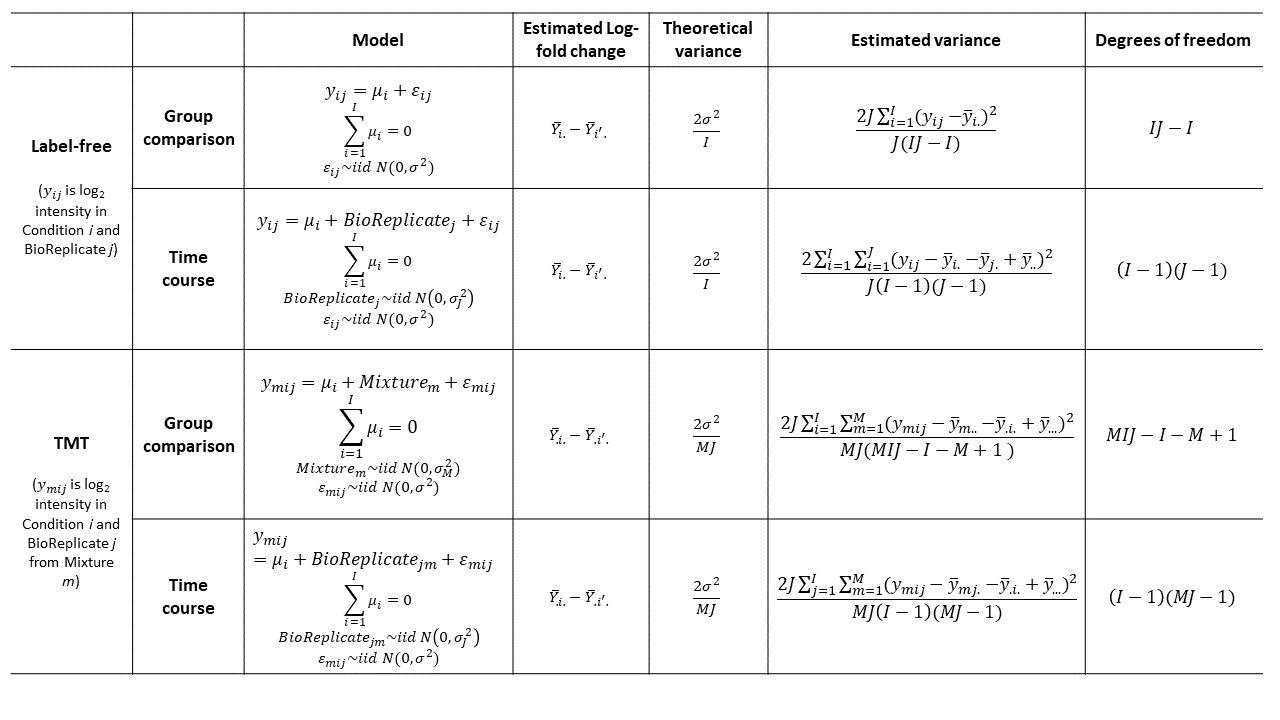
\includegraphics[width=1.2\textwidth]{sim_new/Statistical_inference}}%
\caption{Different models that are fit depending on the experimental design. Models are fit for Label-free and TMT acquisition methods, as well as group comparison and time course experimental designs. The estimation of standard error and degrees of freedom for each model is shown. \label{fig:statistical_inference}}
\end{figure}

%The standard error and degrees of freedom are estimated separately for both the PTM and unmodified protein models. Once this is done we can use these these values to calculate the sample size and perform power analysis. Given $q$, the desired false discovery rate, $\beta$, the average Type II error rate, $m_0 / (m_0 + m_1)$, the fraction of truly differentially modified PTM sites in the comparison. The minimal number of replicates is determined by the variance of the estimated log-fold change $\mathrm{SE}^{2}(\hat{\Delta})$ as
%\[
%\mathrm{SE}^{2}(\hat{\Delta}) = \left[ \left( \hat{\sigma}_{\gamma^{\ast}}^{2} + \hat{\sigma}_{\gamma}^{2} \right) \right]
%\leq \left( \frac{\Delta}{t_{1-\beta, df} + t_{1-\alpha /2, df}} \right)^{2},
%\]
%Where 
%\[
%\alpha = (1 - \beta) \cdot \frac{q}{1 + (1-q) \cdot m_0 / m_1},
%\]
%and $t_{1-\beta, df}$ and $t_{1-\alpha /2, df}$ are the $100(1-\beta)^{\text{th}}$ and the $100(1-\alpha /2)^{\text{th}}$ percentiles of the $t$ distribution. The degrees of freedom are estimated for the appropriate model using restricted maximum likelihood.

\clearpage
%%%%%%%%%%%%%%%%%%%%%%%%%%%%%%%%%%%%%%%%%%%%%%%%%%%%%%%%%%%%%%%%
\section{Experimental datasets}
\label{sec:experiments}
\subsection{Experiments with known ground truth}
\label{sec:sim}

The proposed statistical approach was evaluated and compared to the $t$-test and Limma methods using computer simulations. Specifically, their statistical properties with respect to protein-level adjustment and real world experimental conditions were evaluated.


%%%%%%%%%%%%%%%%%%%%%%%%%%%%%%%%%%%%%%%%%%%%%%%%%%%%%%%%%%%%%%%%
\subsubsection{Computer simulation}
\label{sec:comp_sim}
Differential levels of modified peptides may be due to differential modifications and/or changes in protein abundance. Approaches without considering protein-level adjustment lose track of an important aspect in interpreting observed changes in PTM abundance, which may result in misleading conclusions. To highlight the necessity of the adjustment, we compared six different approaches as follows: a) proposed approach, b) proposed approach without adjusting for unmodified peptides c) $t$-test (with adjustment), d) $t$-test (no adjustment), e) Limma (with adjustment), and f) Limma (no adjustment).

In experiments of complex designs, multiple inter-related conditions are often compared together. The proposed approach and Limma leverage measurements in all conditions for the inference of the underlying abundance, whereas $t$-test uses measurements from the two conditions being compared. To highlight this distinction, multiple conditions of data were generated. While multiple conditions were generated, all comparisons were still made with the same fold change between conditions ($0.75$). This ensured that all peptides were differentially abundant by the same amount and the only difference in calculations was using more conditions in the modeling.

%%%%%%%%%%%%%%%%%%%%%%%%%%%%%%%%%%%%%%%%%%%%%%%%%%%%%%%%%%%%%%%%
\subsubsection{Dataset 1 : Computer simulation 1 - Label-free}
\label{sec:dataset1}
In the first simulation an experiment with many features per PTM and unmodified protein was created. Additionally this simulation contained no missing data. These attributes are not representative of a real experiment, but provide a baseline for model performance.

\begin{itemize}
\item Mean of log-intensity: $25$
\item Standard deviations of log-intensities for modified and unmodified peptides: $0.2$, $0.3$
\item Difference in PTM abundance between conditions: $0$, $0.75$, $1.5$, $2.25$
\item Difference in protein abundance between conditions: $0$, $0.75$, $1.5$, $2.25$
\item Number of replicates: $2$, $3$, $5$, $10$
\item Number of conditions: $2$, $3$, $4$
\item Number of realizations: $1000$
\item Number of features per PTM: $10$
\item Number of features per unmodified protein: $10$
\item Missing data: no missing value
\end{itemize}

The results are summarized from Figure \ref{fig:sim1_fpr} to Figure \ref{fig:sim1_recall}. These results include the false discovery rate with and without adjusting for changes in unmodified protein abundance, false positive rate, and overall accuracy. Additionally, the results are compared to simulation 2 described in the next section.


\subsubsection{Dataset 2 : Computer simulation 2 - Label-free missing values and low features}
\label{sec:dataset2}

In the second simulation we introduced limited feature observations per PTM as well as masking a portion of the observation to simulate missing values. This is more in line with what we would expect in a biological experiment and provides a more realistic expectation of model performance. The number of PTM features and missing data percentage where determined by looking at the features and missing data in the biological experiments in this paper.

\begin{itemize}
\item Mean of log-intensity: $25$
\item Standard deviations of log-intensities for modified and unmodified peptides: $0.2$, $0.3$
\item Difference in PTM abundance between conditions: $0$, $0.75$, $1.5$, $2.25$
\item Difference in protein abundance between conditions: $0$, $0.75$, $1.5$, $2.25$
\item Number of replicates: $2$, $3$, $5$, $10$
\item Number of conditions: $2$, $3$, $4$
\item Number of realizations: $1000$
\item Number of features per PTM: $2$
\item Number of features per unmodified protein: $10$
\item Missing data: 20\% of the observations for PTMs and Proteins were masked with NA at random
\end{itemize}

The results are summarized from Figure \ref{fig:sim2_recall} to Figure \ref{fig:fc_boxplot}.

\begin{figure}[h!]
\centering
 \begin{subfigure}{\textwidth}
  \centering
	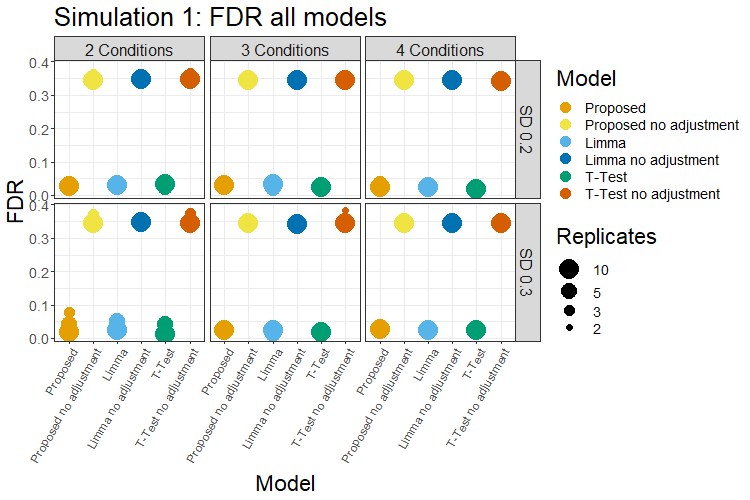
\includegraphics[width=.8\textwidth]{sim_new/sim1_FDR_all_models}\\
	\caption{All the considered methods in simulation 1 correctly calibrated FDR  when adjusting for changes in protein abundance. In comparison, the methods without accounting for the protein-level changes resulted in off-target, high false discovery rates. The performance of the models without adjustment was much lower than those with adjustment, thus only models with adjustment are compared going forward.}
 \end{subfigure}
 \begin{subfigure}{\textwidth}
  \centering
	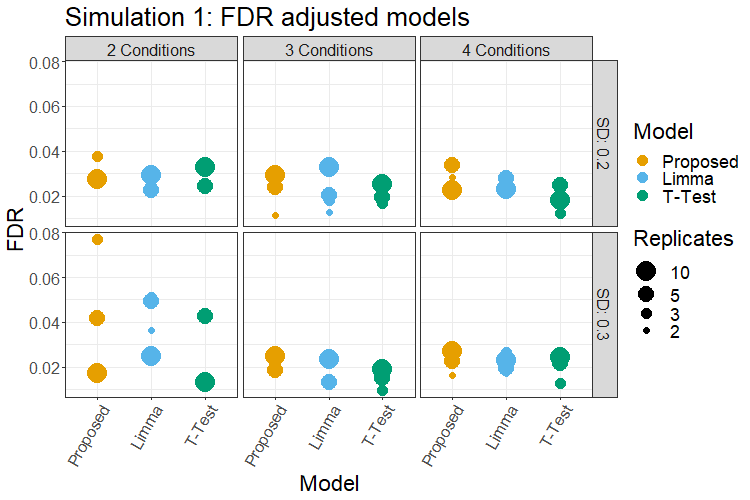
\includegraphics[width=.8\textwidth]{sim_new/sim1_FDR}
	\caption{The considered methods with protein adjustment were compared in detail. All three methods with adjustment generally performed similarly in terms of FDR.}
 \end{subfigure}
 \caption{FDR of Simulation 1.}
\label{fig:sim1_fpr}
\end{figure}

\begin{figure}[h!]
\centering
 \begin{subfigure}{\textwidth}
  \centering
	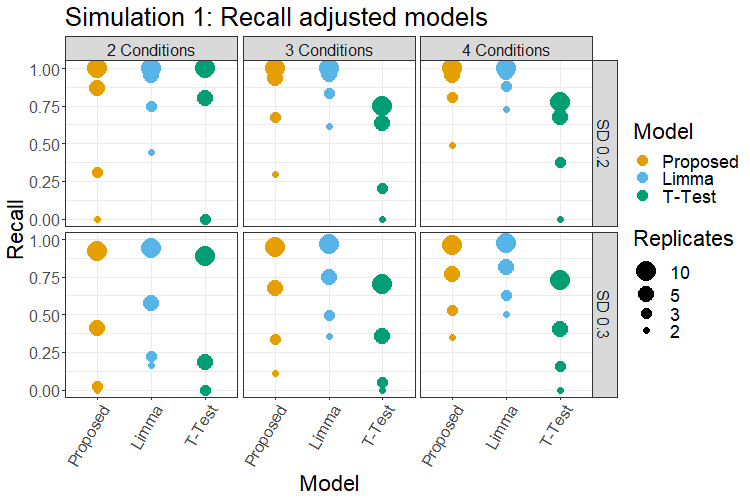
\includegraphics[width=.8\textwidth]{sim_new/sim1_Recall}\\
	\caption{All methods with adjustment were compared by comparing recall in simulation 1. Limma performed the strongest here when the number of replicates were low. At higher replicates the performance of the proposed methods and Limma were comparable. $t$-test clearly performed worse across all methods.}
 \end{subfigure}
 \begin{subfigure}{\textwidth}
  \centering
	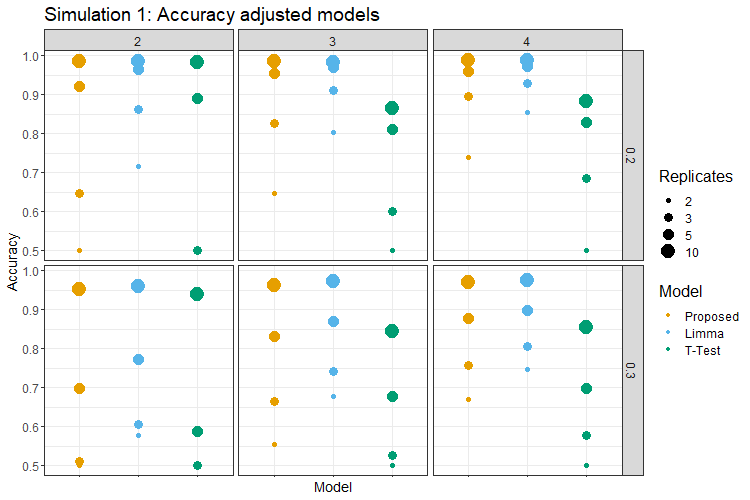
\includegraphics[width=.8\textwidth]{sim_new/sim1_accuracy}
	\caption{The overall accuracy plot mimicked the observations in the recall plot. Limma performed strongest when replicates were low, but was comparable to the proposed method with more replicates.}
 \end{subfigure}
\caption{Recall and Accuracy results of Simulation 1.}
\label{fig:sim1_recall}
\end{figure}

\begin{figure}[h!]
\centering
	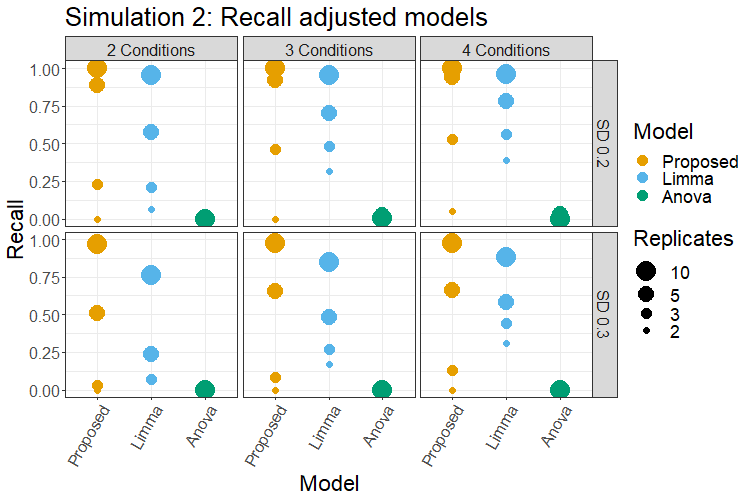
\includegraphics[width=.8\textwidth]{sim_new/sim3_Recall}
	\caption{}
\caption{Recall results of Simulation 2. The advantage of using the proposed approach were apparent when looking at simulation 2, which included limited observations and the presence of missing values. In the case of recall the proposed method performed stronger than Limma and t-test in nearly every model. Even at lower replicates the proposed method still outperformed Limma. Again the lowest performing method was $t$-test.}
\label{fig:sim2_recall}
\end{figure}

\begin{figure}[h!]
\centering
 \begin{subfigure}{\textwidth}
 \centering
	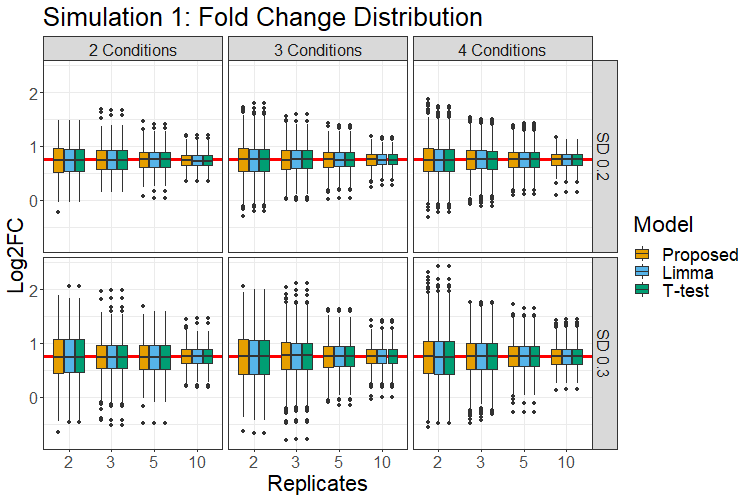
\includegraphics[width=.8\textwidth]{sim_new/sim1_FC_boxplot}
	\caption{In simulation 1 all considered methods correctly estimated the fold change between conditions, with a median fold change estimation of .75. The distributions around the median were also consistent across all methods.}
 \end{subfigure}
 \begin{subfigure}{\textwidth}
  \centering
	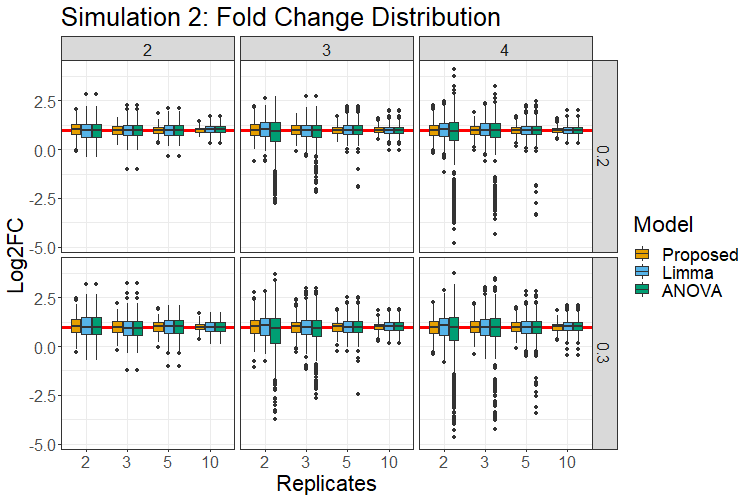
\includegraphics[width=.8\textwidth]{sim_new/sim3_FC_boxplot}
	\caption{In simulation 2 all methods correctly estimated the fold change with a median log change of .75. The proposed method in this simulation had a visibly tighter distribution around the median. Both Limma and $t$-test showed a wider range around the fold change. The inner quartile range of the Proposed method was on average 10.4\% smaller than t-test and 21.8\% smaller than Limma.}
 \end{subfigure}
\caption{Fold change distribution comparison between Simulations 1 and 2.}
\label{fig:fc_boxplot}
\end{figure}

\clearpage
%%%%%%%%%%%%%%%%%%%%%%%%%%%%%%%%%%%%%%%%%%%%%%%%%%%%%%%%%%%%%%%%
\subsubsection{Dataset 3 : SpikeIn benchmark - Ubiquitination - Label-free}
\label{sec:benchmark}

%A custom designed experiment with labeling was used to assess the performance of the proposed method in a real experimental setting. Heavy-labeled KGG modified peptides were used as spike-in peptides. The spike-in peptides were mixed with human lysate to create four mixture conditions. Two sets of data were acquired for each mixture: KGG enriched + LC-MS, and LC-MS only. The KGG enriched dataset included the spike-in peptides, as well as modified and unmodified human lysate. The LC-MS dataset included only unmodified peptides. The spike-in peptides have a known fold change between conditions and are expected to be differential in most cases. Additionally, background E coli lysate was used to normalize total protein levels prior to the enrichment and global protein profiling. The background lysate was treated as controls and are not expected to be differential in any comparison.

%\begin{figure}[h!]
%\centering
%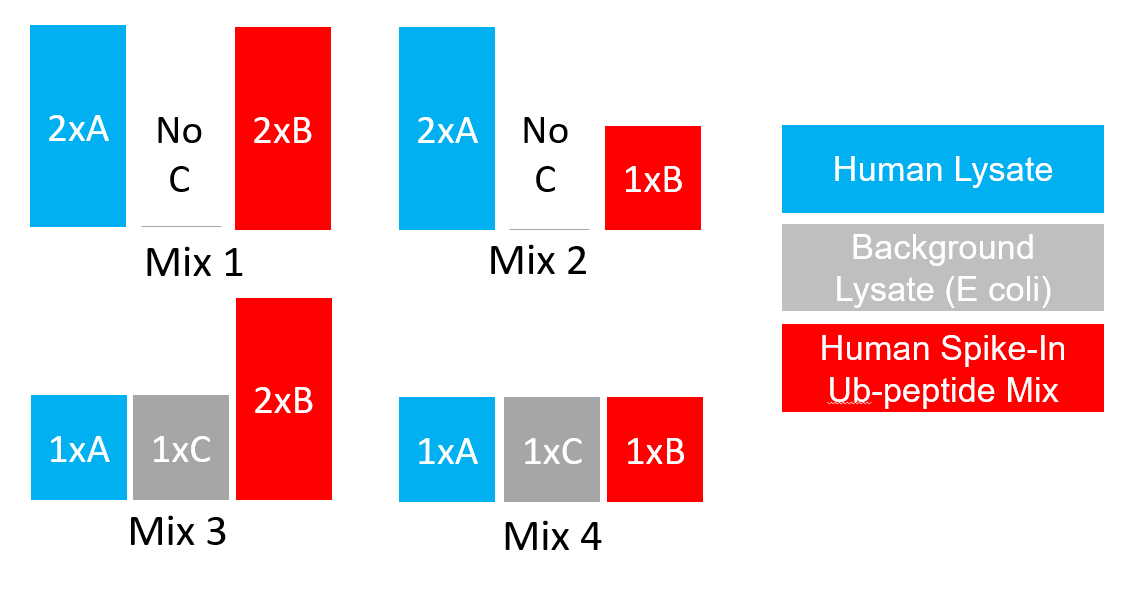
\includegraphics[width=.8\textwidth]{sim_new/SpikeIn_Overview}
%\caption{An overview of the spike-in benchmark experimental design. The corresponding levels of spike-in peptide, human lysate, and background lysate for each mixture are shown. The spike-in peptide levels are adjusted for the human lysate levels. For example, the true spike-in abundance of mixture 1 is entirely accounted for by human lysate, whereas mix 2 has double the amount human lysate compared to spike-in abundance. When comparing mix 1 vs mix 2 we would expect to see a log fold change of -1. In this way we know the expected log fold change between mixture comparisons. \label{fig:spikein_overview}}
%\end{figure}

Again we consider three different methods and assess their performance: the method proposed in this paper, Limma, and two sample $t$-test. All methods are analyzed after adjusting for changes in overall protein level. The results are summarized from Figure \ref{fig:spike_volcano_msstats} to Figure \ref{fig:spike_stat}, including volcano plots, model summary statistics, and fold change analysis.

\begin{figure}[h!]
\centering
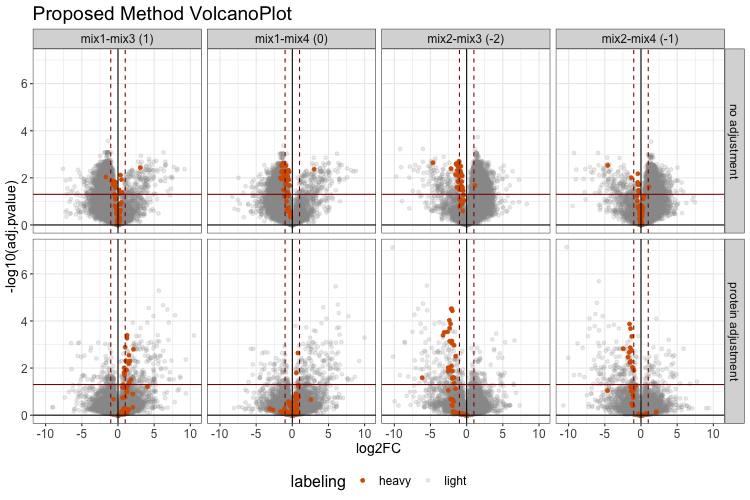
\includegraphics[width=1\textwidth]{sim_new/spike_in_msstatsptm_volcano}
\caption{The modeling results of the proposed method both before and after adjustment. The spike-in peptides are colored red and the background peptides are colored grey. All grey peptides are expected to be insignificant. Using the proposed method to model the benchmark experiment, the spike-in peptides (colored red) did not follow the expected log fold change before adjustment. After adjusting for changes in overall protein abundance the spike-in peptides were more in line with expectation. Additionally the background grey colored peptides showed many false positives before adjustment. After adjustment these false positives were decreased considerably. \label{fig:spike_volcano_msstats}}
\end{figure}

\begin{figure}[h!]
\centering
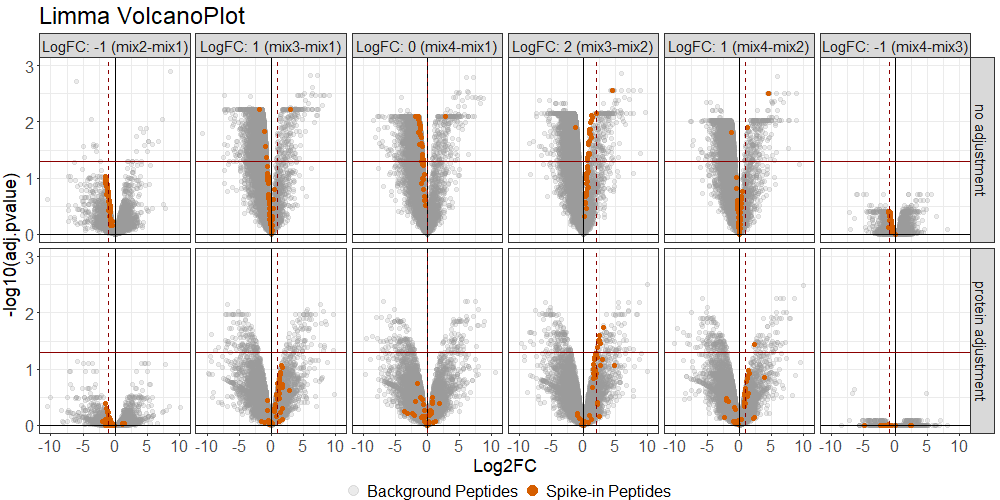
\includegraphics[width=.85\textwidth]{sim_new/spike_in_limma_volcano}
\caption{When modeling the experiment with the Limma method, the spike-in peptides again follow the expected log fold change better after adjusting for changes in protein level. However, while the fold change was more accurate, the majority of spike-in peptides did not have a significant adjusted pvalue. In this case, the known differential peptides were missed by the model. In terms of false positives, the results were very similar to the proposed method, with many false positives before adjustment and fewer after. \label{fig:spike_volcano_limma}}
\end{figure}

\begin{figure}[h!]
\centering
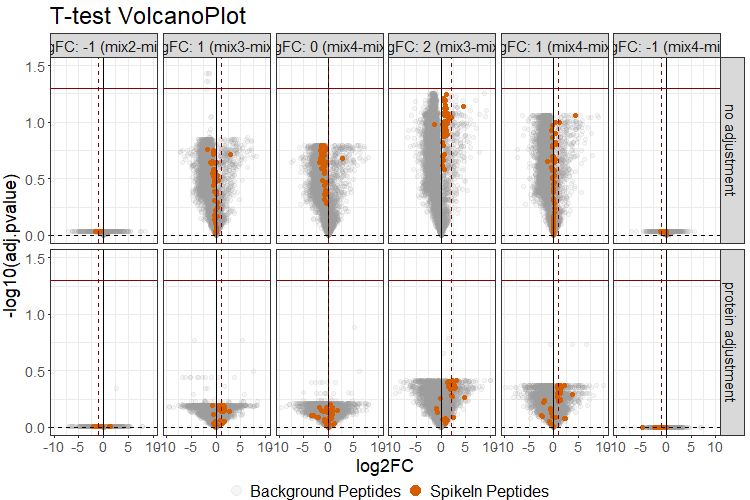
\includegraphics[width=.85\textwidth]{sim_new/spike_in_ttest_volcano}
\caption{Using the two sample $t$-test, none of the comparisons either before or after adjustment show any significant peptides. With that being said, the fold change of the spike-in peptides was much closer to expectation after adjusting for global protein abundance. \label{fig:spike_volcano_ttest}}
\end{figure}

\begin{figure}[h!]
\centering
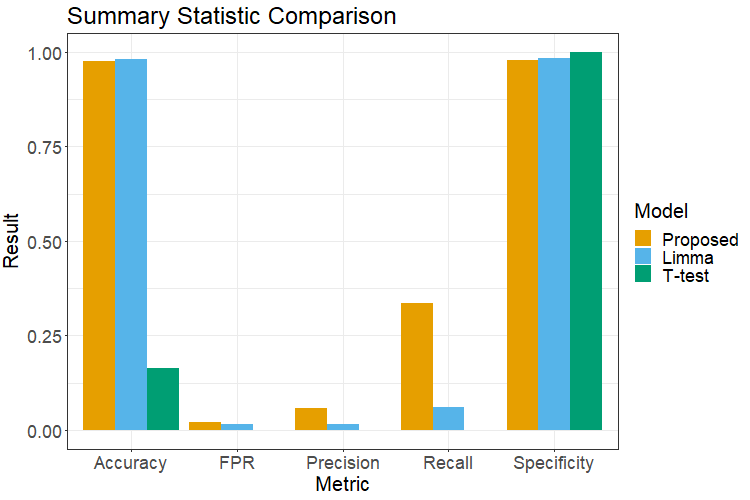
\includegraphics[width=.85\textwidth]{sim_new/spike_in_statistic_comparison}
\caption{Comparing the summary statistics between methods, the proposed method performed the strongest. In terms of accuracy and specificity the three methods were close, with Limma and $t$-test showing slightly higher values. Accuracy and specificity were dominated by the large number of true negatives (background peptides) compared to the true positives (spike-in peptides). In terms of recall, the proposed approach out performed the other two methods, showing that it correctly labeled the most spike-in peptides. \label{fig:spike_stat}}
\end{figure}

\clearpage
%%%%%%%%%%%%%%%%%%%%%%%%%%%%%%%%%%%%%%%%%%%%%%%%%%%%%%%%%%%%%%%%
\subsection{Biological investigations}
\label{sec:bio_investigations}

\subsubsection{Dataset 4 : Human - Ubiquitination - 1mix-TMT~\cite{LUCHETTI2021}}
\label{sec:ipah}

The experimental design can be seen in Table~\ref{table:ipah_design}.

\begin{table}[h!]
\centering
\begin{tabular}{| c | c | c |}
\hline
 Condition & BioReplicate & Channel \\ [0.5ex]
 \hline\hline
 Dox1hr & Dox1hr\_1 & 127C\\
 \hline
 Dox2hr & Dox2hr\_1 & 128N\\
\hline
 Dox2hr & Dox2hr\_2 & 130C\\
\hline
 Dox4hr & Dox4hr\_1 & 128C\\
\hline
 Dox4hr & Dox4hr\_2 & 131C\\
\hline
 Dox6hr & Dox6hr\_1 & 129N\\
\hline
 Dox6hr & Dox6hr\_2 & 131N\\
\hline
 NoDox0hr & NoDox0hr\_1 & 126C\\
\hline
 NoDox0hr & NoDox0hr\_2 & 129C\\
\hline
 NoDox6hr & NoDox6hr\_1 & 127N\\
\hline
 NoDox6hr & NoDox6hr\_2 & 130N\\
\hline

\end{tabular}
\caption{The experimental design of Dataset 4}
\label{table:ipah_design}
\end{table}

A model was fit for the total protein and ubiquitination separately. The model formula can be seen below.

$$Y_{mcb} = \mu + Condition_c + Subject_{mcb} + \epsilon_{mcb}$$

$$\sum_{c=1}^C{Condition_c} = 0 ,\: Subject_{mcb} ~ \sim N(0, \sigma^2_S) ,\: \epsilon_{mcb} ~ \sim N(0, \sigma^2)$$

The results of the proposed method to this experiment can be seen in Figure \ref{fig:ipah_figures}.

\begin{figure}[h!]
\centering
 \begin{subfigure}{\textwidth}
 \centering
	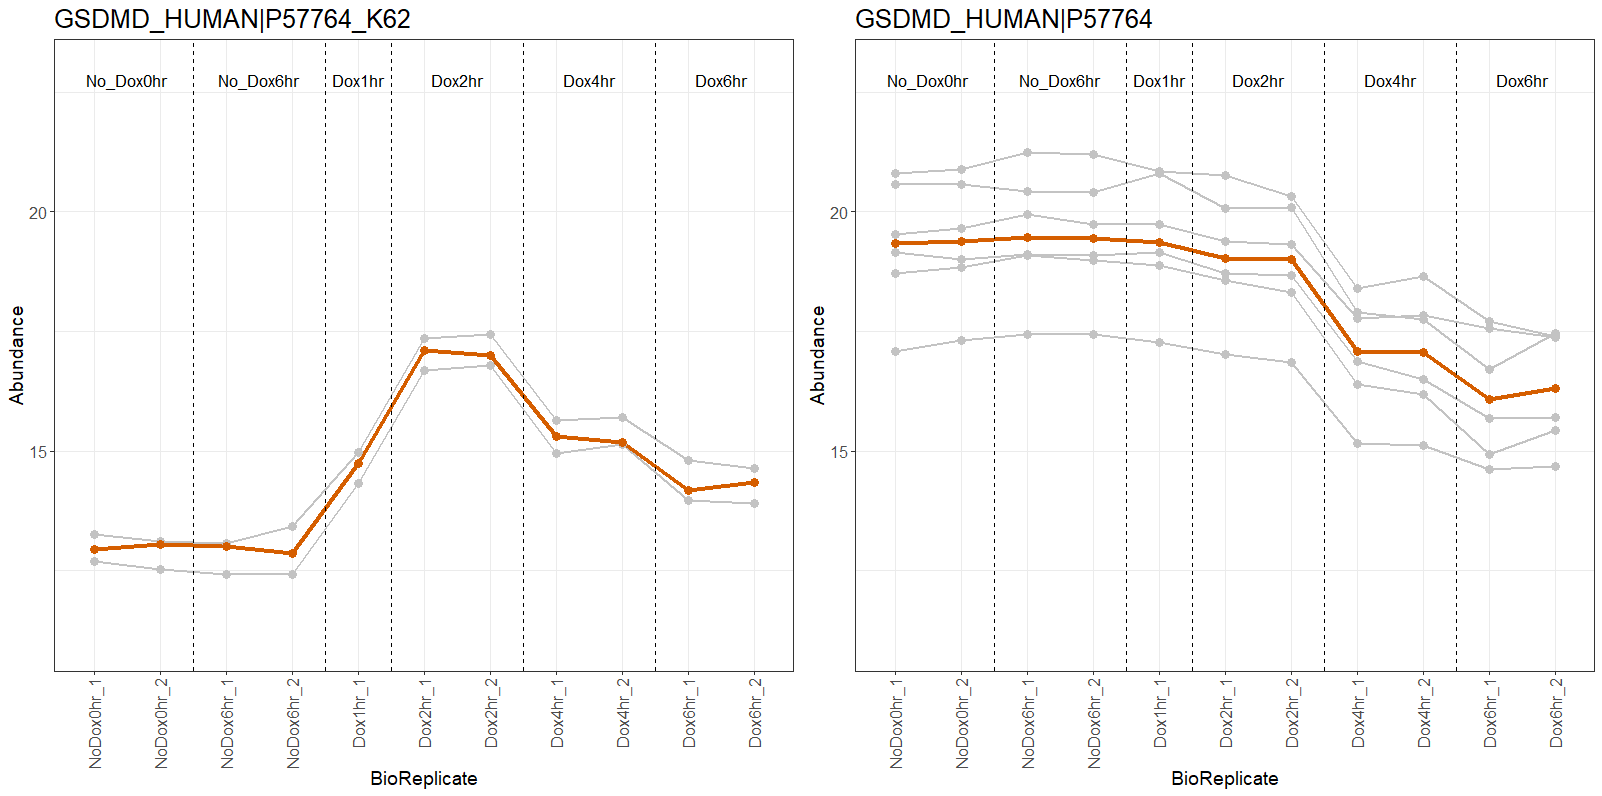
\includegraphics[width=.9\textwidth]{sim_new/IpaH_prof_plot}
	\caption{Here the global profiling of protein $GSDMD\_HUMAN|P57764$ with the ubiquitination of the protein at site $K62$ was compared. The individual PSM features areshown in grey, while the feature summarization is shown in red. The summary of the modification and global protein showed that the conditions followed different trends. Specifically, there appeared to be no change in abundance between Dox1hr and Dox4hr in the modified plot, however there was a large negative change in the unmodified plot. This indicates the modification was confounded with changes in the unmodified protein.}
 \end{subfigure}
 \begin{subfigure}{\textwidth}
 \centering
	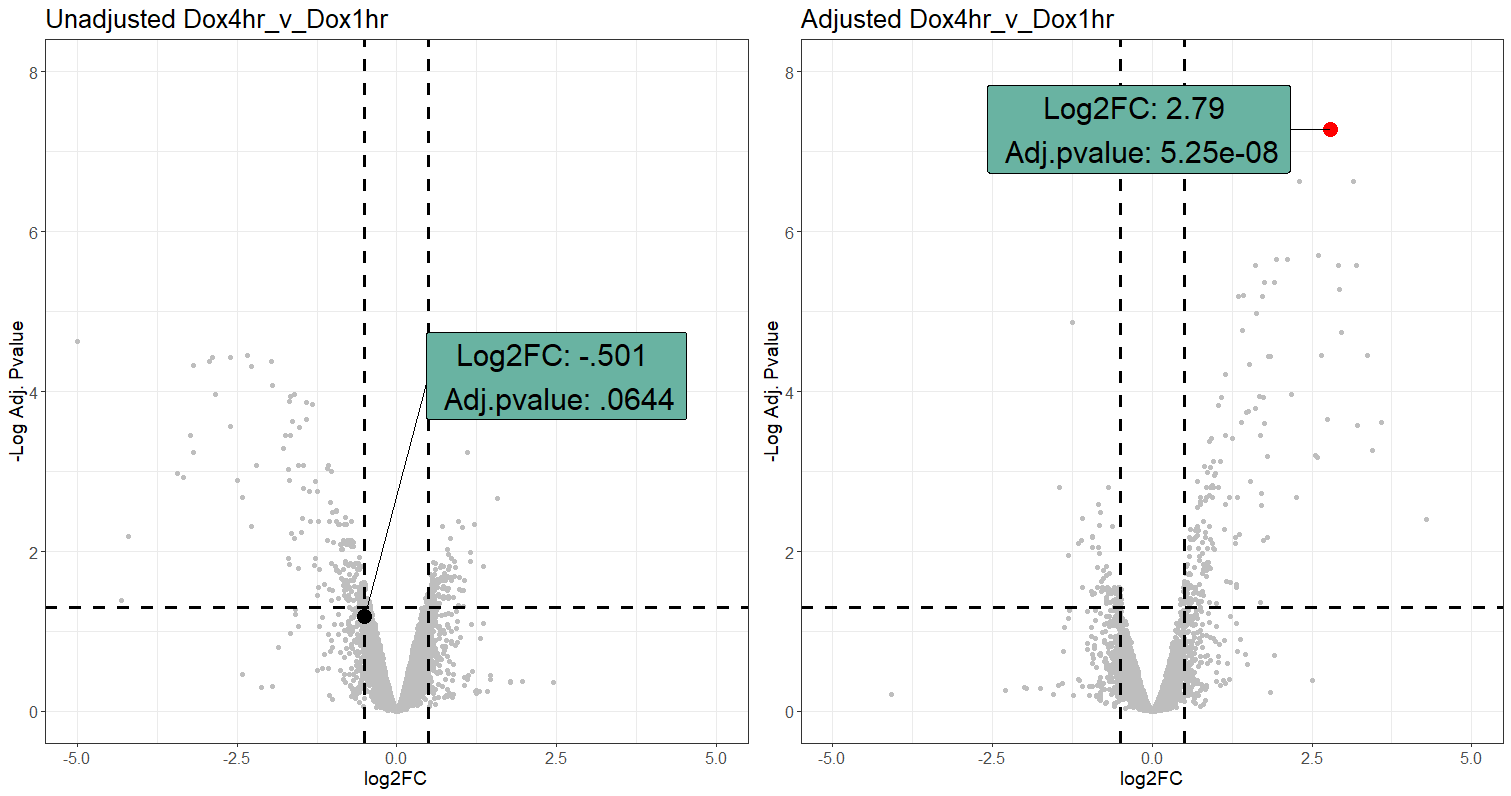
\includegraphics[width=.9\textwidth]{sim_new/IpaH_volcano_plot}
	\caption{Volcano plots of Dox4hr vs Dox1hr both before and after protein adjustment. The $GSDMD\_HUMAN|P57764\_K62$ modification is highlighted. Before adjustment the modification had a small fold change and insignificant adjusted pvalue. After adjustment the fold change was much larger and the adjusted pvalue was significant. In this case the proposed method allowed us to identify a differential modified peptide that could have otherwise been missed.}
 \end{subfigure}
\caption{Summary plots for modification of protein GSDMD at site K62.}
\label{fig:ipah_figures}
\end{figure}

\clearpage
\subsubsection{Dataset 5 : Mouse - Phosphorylation - 2mix-TMT}
\label{sec:shigella}

In this study, the correlation between the gene Atg16L1 and killing of Shigella flexneri (S.flexneri) was assessed~\cite{Maculins}. Multiplex proteomics was used to quantify the abundance of total protein, phosphorylation, and ubiquitination in wild type (WT) and ATG16L1-deficient (cKO) samples, uninfected and uninfected with S.flexneri. The abundance of total protein and post-translation modifications were quantified at three time points, uninfected, early infection (45-60 minutes), and late infection (3-3.5 hours). Quantifying the total protein along with the post-translational modifications allowed us to adjust for changes in total protein and see the true impact of the site specific modifications. Two mixtures using 11-plex were ran over the six conditions. The six conditions were split between 11 channels leading to an unbalanced experimental design. Each mixture contained two replicates per early and late WT and KO conditions. Mixture one contained one replicate of uninfected WT and two replicates of uninfected KO. Mixture two contained one replicate of uninfected KO and two uninfected WT. The experimental design can be seen in Table~\ref{table:shigella_design}.

\begin{table}[h!]
\centering
\begin{tabular}{|c | c c | c c | c|}
\hline
 & \multicolumn{2}{c}{Mixture 1} & \multicolumn{2}{c}{Mixture 2} & Condition \\ [0.5ex]
 \hline\hline
 Uninfected & 128C & & 128C & 131C & \\
 \hline
Early (1 Hour) & 126C & 129C & 126C & 129C & WT \\
\hline
Late (3 Hour) & 127C & 130C & 127C & 130C & \\
\hline
Uninfected & 129N & 131C & 129N & & \\
\hline
Early (1 Hour) & 127N & 130N & 127N & 130N & KO \\
\hline
Late (3 Hour) & 128N & 131N & 128N & 131N & \\
\hline

\end{tabular}
\caption{The experimental design of Dataset 5}
\label{table:shigella_design}
\end{table}

A model was fit for the total protein, phosphorylation, and ubiquitination separately, as described previously for TMT experiments. The model formula can be seen below.

$$Y_{mcb} = \mu + Mixture_m + Condition_c + Subject_{mcb} + \epsilon_{mcb}$$

$$Mixture_m ~ \sim N(0, \sigma^2_M) ,\: \sum_{c=1}^C{Condition_c} = 0 ,\: Subject_{mcb} ~ \sim N(0, \sigma^2_S) ,\: \epsilon_{mcb} ~ \sim N(0, \sigma^2)$$

The results of the proposed method to this experiment can be seen in Figure \ref{fig:No_Diff_Shigella_PTM} and Figure \ref{fig:Diff_Shigella_PTM}.


\begin{figure}[h!]
\centering
 \begin{subfigure}{\textwidth}
 \centering
	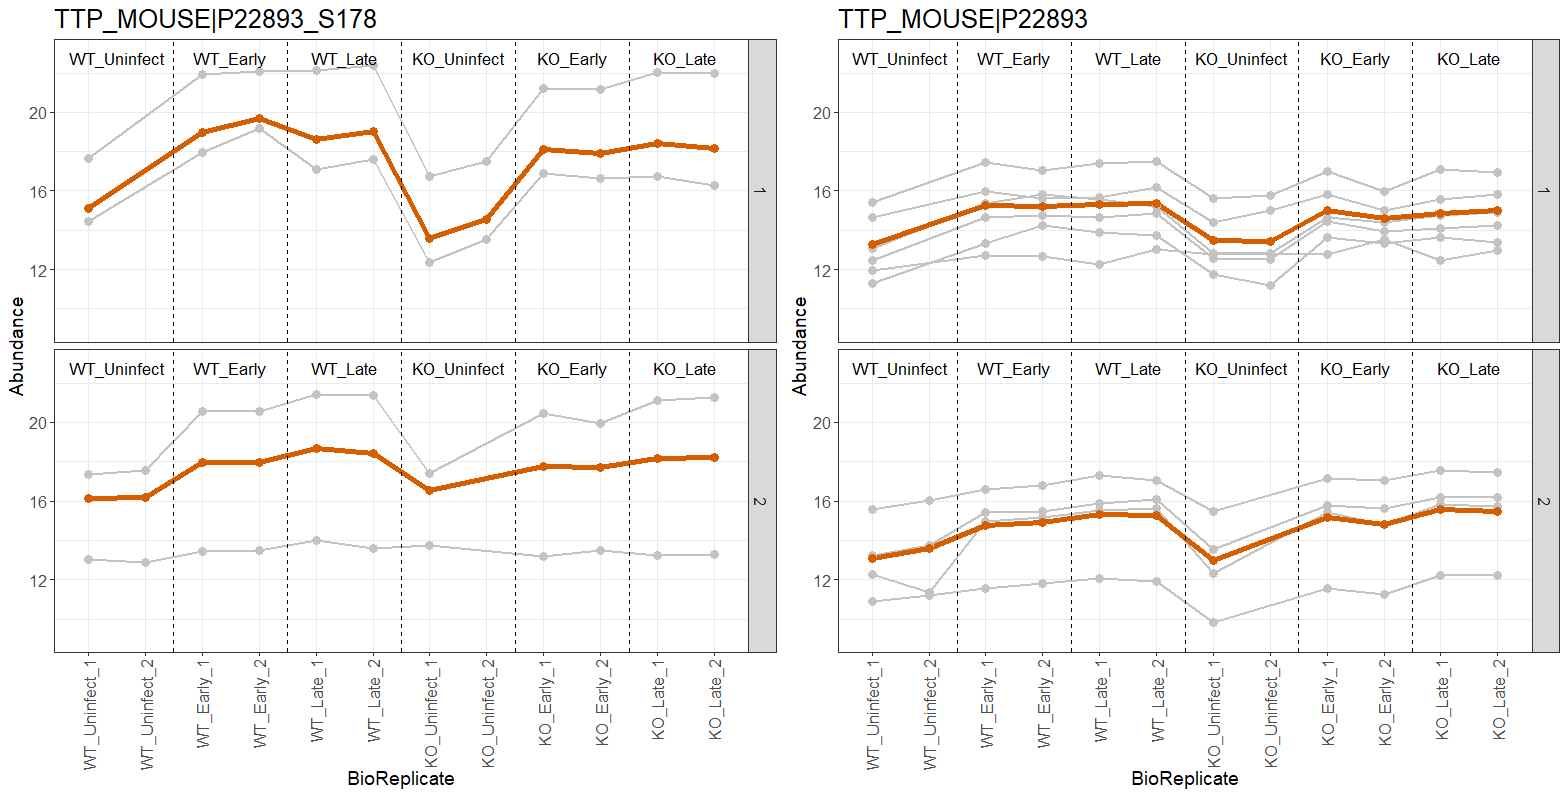
\includegraphics[width=.95\textwidth]{sim_new/No_Difference_Shigella_Profile_Plot}
	\caption{The global profiling of protein $TTP\_MOUSE|P22893$ with the modification of the protein at site $S178$ was compared. The individual PSM features are shown in grey, while the feature summarization is shown in red. The summary of the modification and global protein showed that the conditions followed the same trend. Specifically, there was a positive adjustment in abundance when comparing WT\_Uninfect to WT\_Late in both the modification and global profiling run. This indicated the movement is driven by changes in global protein.}
 \end{subfigure}
 \begin{subfigure}{\textwidth}
 \centering
	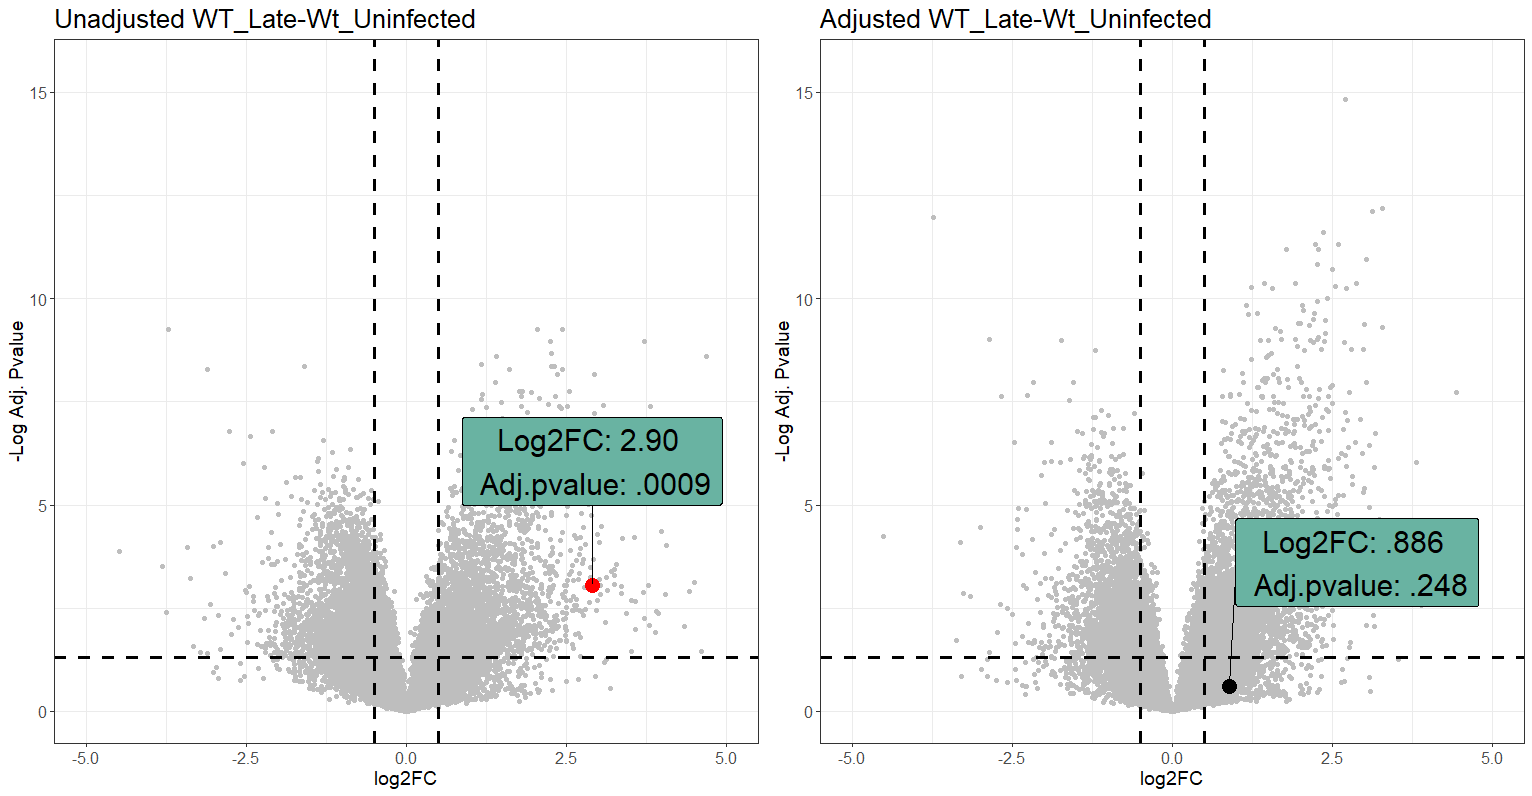
\includegraphics[width=.9\textwidth]{sim_new/No_Difference_Shigella_Volcano}
	\caption{Volcano plots of WT\_Late vs WT\_Uninfect both before and after protein adjustment. The $TTP\_MOUSE|P22893\_S178$ modification is highlighted. Before adjustment the modification had a large fold change and significant adjusted pvalue. After adjustment the fold change was much smaller and the adjusted pvalue was insignificant.}
 \end{subfigure}
\caption{Summary plots for modification of protein TTP at site S178.}
\label{fig:No_Diff_Shigella_PTM}
\end{figure}

\begin{figure}[h!]
\centering
 \begin{subfigure}{\textwidth}
 \centering
	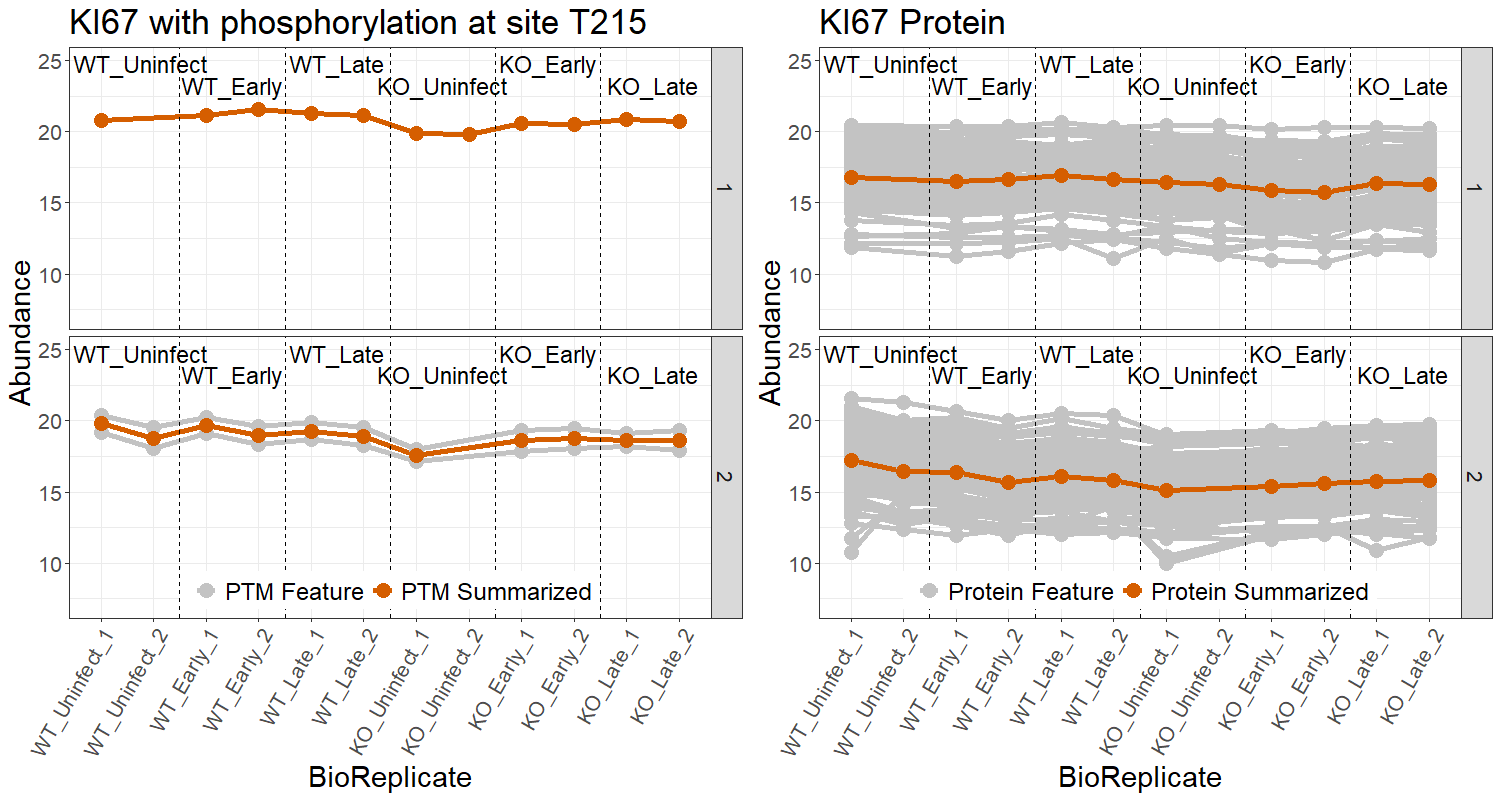
\includegraphics[width=.9\textwidth]{sim_new/Difference_Shigella_Profile_Plot}
	\caption{The global profiling of protein $KI67\_MOUSE|E9PVX6$ with the modification at site $T215$ was compared. In this case the modification and global protein appeared to show small or no difference between conditions, however after adjusting for change in global protein abundance, the modification was statistically significant. Additionally, this profile plot showed the large difference in available features between modified peptides and global proteins.}
 \end{subfigure}
 \begin{subfigure}{\textwidth}
 \centering
	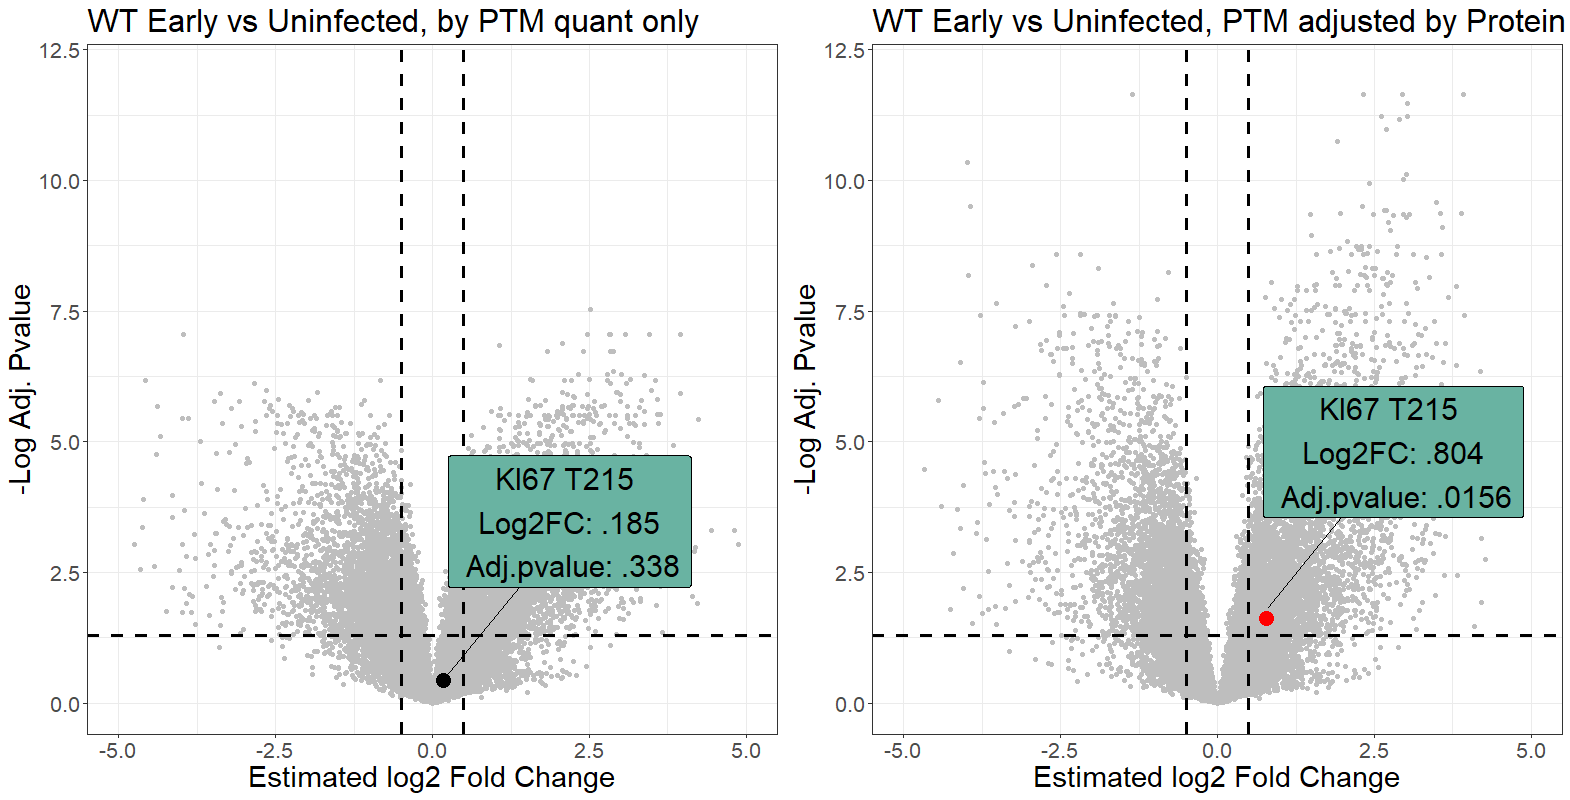
\includegraphics[width=.9\textwidth]{sim_new/Difference_Shigella_Volcano}
	\caption{The volcano plot of the WT\_Uninfect and WT\_Early comparison showed the specifics of the adjustment. The modification looked to be flat, with a log fold change of $.185$, while the global profiling showed a small negative fold change of $-.619$. While both exhibit small changes, when combined we saw a log fold change of $.804$ and adjusted p-value of $.0156$.}
 \end{subfigure}
 \caption{Summary plots for modification of protein KI67 at site T215.}
\label{fig:Diff_Shigella_PTM}
\end{figure}

\clearpage

\subsubsection{Dataset 6 : Human - Ubiquitination - Label-free no global profiling run}
\label{sec:usp30}

This experiment looked into the relationship between USP30 and protein kinase PINK1, and their association with Parkinson's Disease. Ubiquitination site profiling was performed and the modified site abundance was analyzed. Four conditions were tested with two biological replicates per condition. The conditions were as follows: CCCP, USP30 overexpression (USP30\_OE), Combo, and Control. Label-free mass spectrometry quantification was used to quantify the abundance of modified peptides. A corresponding mixed effects model was fit per modification and global protein as described previously in this supplementary. The experiment was modeled as a group comparison.

In contrast to other experiments analyzed in this paper, there was no unmodified global protein profiling run performed in this experiment. Once identification and quantification of the Ubiquitinated profiling was performed, peptides which were unmodified were extracted and used in place of a global profiling run. This resulted in a significant lack of overlap between modified and unmodified peptides and low feature counts for the unmodified protein model.

An example profile plot for this experiment can be seen in  Figure \ref{fig:USP30_profile_plot}.

\begin{figure}[h!]
\centering
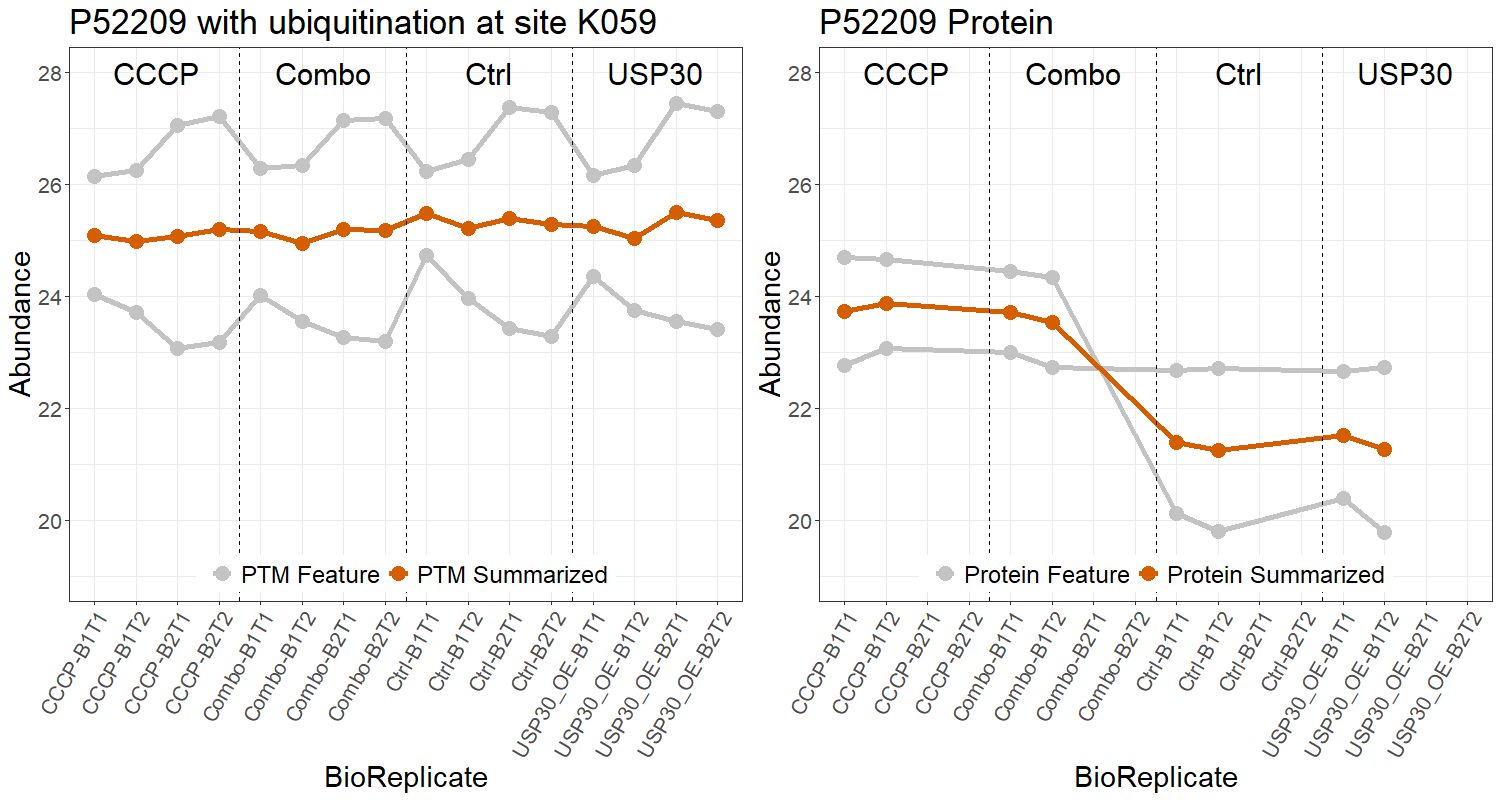
\includegraphics[width=\textwidth]{sim_new/USP30_profile_plot}
\caption{The global profiling of protein $P52209$ with the modification of the protein at site $K059$ was compared. The modification appeared generally unchanged between all conditions, whereas the global profiling run showed the CCCP and Combo conditions had a higher relative abundance compared to the Control and USP30\_OE. This indicated that the modification actually had an effect when comparing CCCP and Combo to Control and USP30\_OE. However it was not entirely clear as one unmodified peptide feature appeared to be changed, while the other did not. This uncertainty was another result of not running a separate global profiling run. With a global profiling run, many unmodified features are generally quantified, removing the uncertainty that comes with low feature counts.}
\label{fig:USP30_profile_plot}
\end{figure}
\clearpage
%%%%%%%%%%%%%%%%%%%%%%%%%%%%%%%%%%%%%%%%%%%%%%%%%%%%%%%%%%%%%%%%
\section{Sample size calculation and power analysis}

\subsubsection*{Noisy PTM measurements benefited from additional biological replicates}

Here we analyzed the sample size needed to achieve a desired statistical power. The proposed approach corrected for confounding between the modified peptide and unmodified protein at the cost of increased variation. This can be seen in the calculation for variance. Increased variation required a larger number of replicates to reach the same power. Thus the statistical power was dependent on the variance from both the modified peptide and unmodifed protein.

We compared the statistical power in experiments with differing numbers of replicates, variance, and fold change for both the modified and unmodified runs. In terms of the number of replicates, we tested scenarios with equal replicates in both the modified and unmodified runs, as well as scenarios where the replicates differed between runs. We used the biological experiments to determine what variance values to test. In datasets 4 and 5 the variance of the PTM was higher than the global protein. In dataset 6 the variance of the PTM and Protein were generally the same. We mimicked these scenarios and analyzed the power of experiments when the PTM variance was higher than the protein and when they were equal. When the PTM and protein were the same we chose a variance of $.15$, whereas when the PTM was higher than the protein we chose a PTM variance of $.2$ and a protein variance of $.1$.

The results of the power and sample size analysis can be seen in Figure \ref{fig:power_sd_combo}. When the variance and replicates were equal, higher replicates predictably lead to higher power. In cases where the replicates were unbalanced, but the variance was still the same, it did not matter if there were more replicates in the modified or unmodified runs. In comparison, with differing variance and equal replicates, higher replicates still lead to higher power. When the replicates were unbalanced and the variance was higher in the PTM, there was more power when more replicates were allocated to the PTM run than the unmodified protein run. The results lead to the takeaway that in cases where the number of replicates have to be limited, it is better to allocate more to the PTM run.

\begin{figure}[h!]
\centering
 \begin{subfigure}{\textwidth}
 \centering
	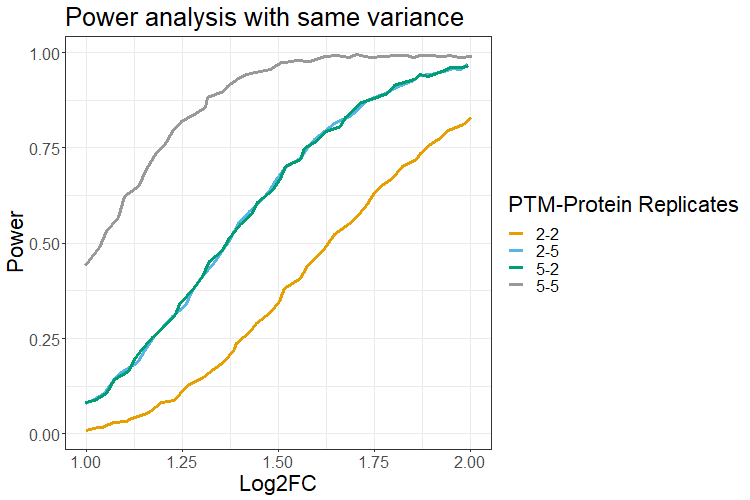
\includegraphics[width=.75\textwidth]{sim_new/same_var_power}
	\caption{The power of an experiment targeting PTMs with the same variance, .15, for the modified and unmodified peptides. Predictably when the replicates were high for both modified and unmodified peptides the power was much higher. Conversely at low replicates for each the power was much lower. With equal variance, it did not matter if the PTM replicates or protein replicates were higher.}
 \end{subfigure}\vspace{-1mm}
 \begin{subfigure}{\textwidth}
 \centering
	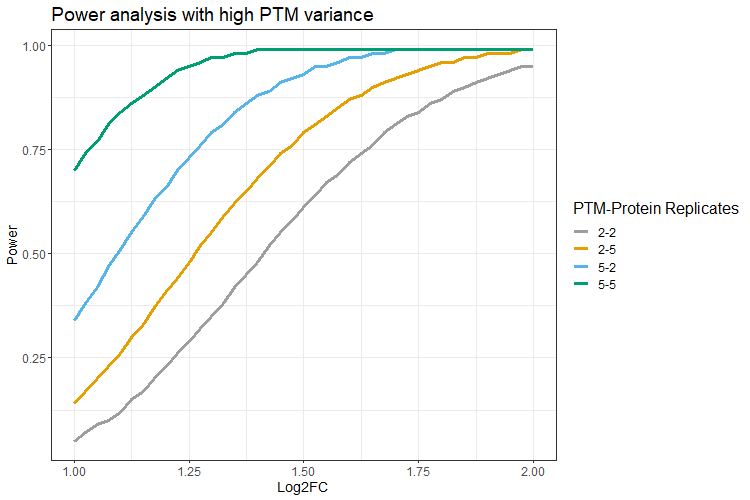
\includegraphics[width=.75\textwidth]{sim_new/high_ptm_var_power}
	\caption{In this chart the variance for the PTM was higher than the unmodified protein. The PTM variance was .2, while the unmodified protein variance was .1. With equal replicates the results were the same as above. When the replicates were not equal, more replicates allocated to the PTM runs lead to higher power.}
 \end{subfigure}\vspace{-1mm}
 \caption{Power analysis of experiments with differing variances.}
\label{fig:power_sd_combo}
\end{figure}

%The proposed approach allows us to calculate the sample size needed to achieve a desired statistical power as described in Section \ref{sec:design}. The proposed method adjusts for the underlying protein abundance in the PTM significance analysis, which corrects the confounding factor with a cost of increased variation. When the variation is increased, the experiment requires a larger number of replicates to reach the same power. Thus the statistical power is dependent on the variance from both the modified peptide and unmodifed protein as well as the number of replicates in both runs.

%We compared the statistical power in experiments with differing numbers of replicates, variance, and fold change for both the modified and unmodified runs. For variance we used the variance from the biological experiments to determine what values to set. In dataset 4 and 5 the variance of the PTM was generally higher than the global protein. In contrast, in dataset 6 the variance of the PTM and Protein was generally the same. Because of this we will analyze the power of our experiments when the PTM variance is higher than the protein, and also when they are the same. For the variance numbers, in the case when the PTM and protein are the same we chose a variance of .15. When the PTM is higher than the protein we chose a PTM variance of .2 and a protein variance of .1. These numbers were derived from the biological experiments in this paper.

%The results of the power and sample size analysis can be seen in \sfigref{fig:power_sd_combo}.

%\begin{figure}[h!]
%\centering
% \begin{subfigure}{\textwidth}
% \centering
%	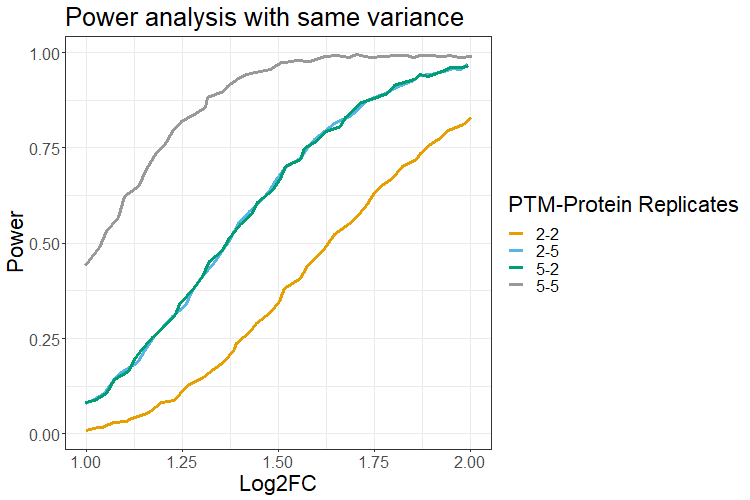
\includegraphics[width=.725\textwidth]{sim_new/same_var_power}
%	\caption{Here we can see the power of an experiment targeting PTMs with the same variance, .15, for the modified and unmodified peptides. Predictably when the replicates are high for both modified and unmodified peptides the power is much higher. Conversely at low replicates for each the power is much lower. The interesting part of this chart is when the replicates are different between runs. With equal variance, it does not matter if the PTM replicates or protein replicates are higher. Both cases result in the same power with equal variance.}
% \end{subfigure}\vspace{-5mm}
% \begin{subfigure}{\textwidth}
% \centering
%	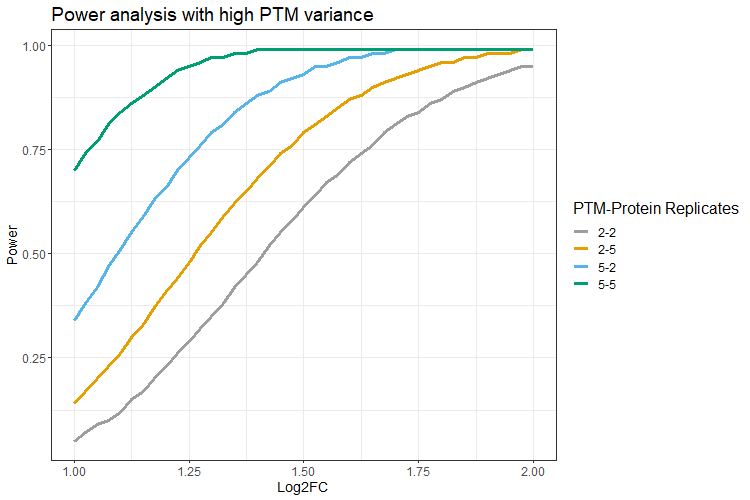
\includegraphics[width=.725\textwidth]{sim_new/high_ptm_var_power}
%	\caption{In this chart the variance for the PTM is higher than the unmodified protein. The PTM variance is .2, while the unmodified protein variance is .1. With equal replicates the results are the same as above, more replicates equals more power. When the replicates are not the same we can clearly see that having more replicates for the PTM leads to more power. It is clearly more important to have high replicates for the PTM run than the unmodified protein, when the PTM variance is higher.}
% \end{subfigure}
% \caption{Power analysis of experiments with differing variances.}
%\label{fig:power_sd_combo}
%\end{figure}


%\begin{figure}[h!]
%\centering
%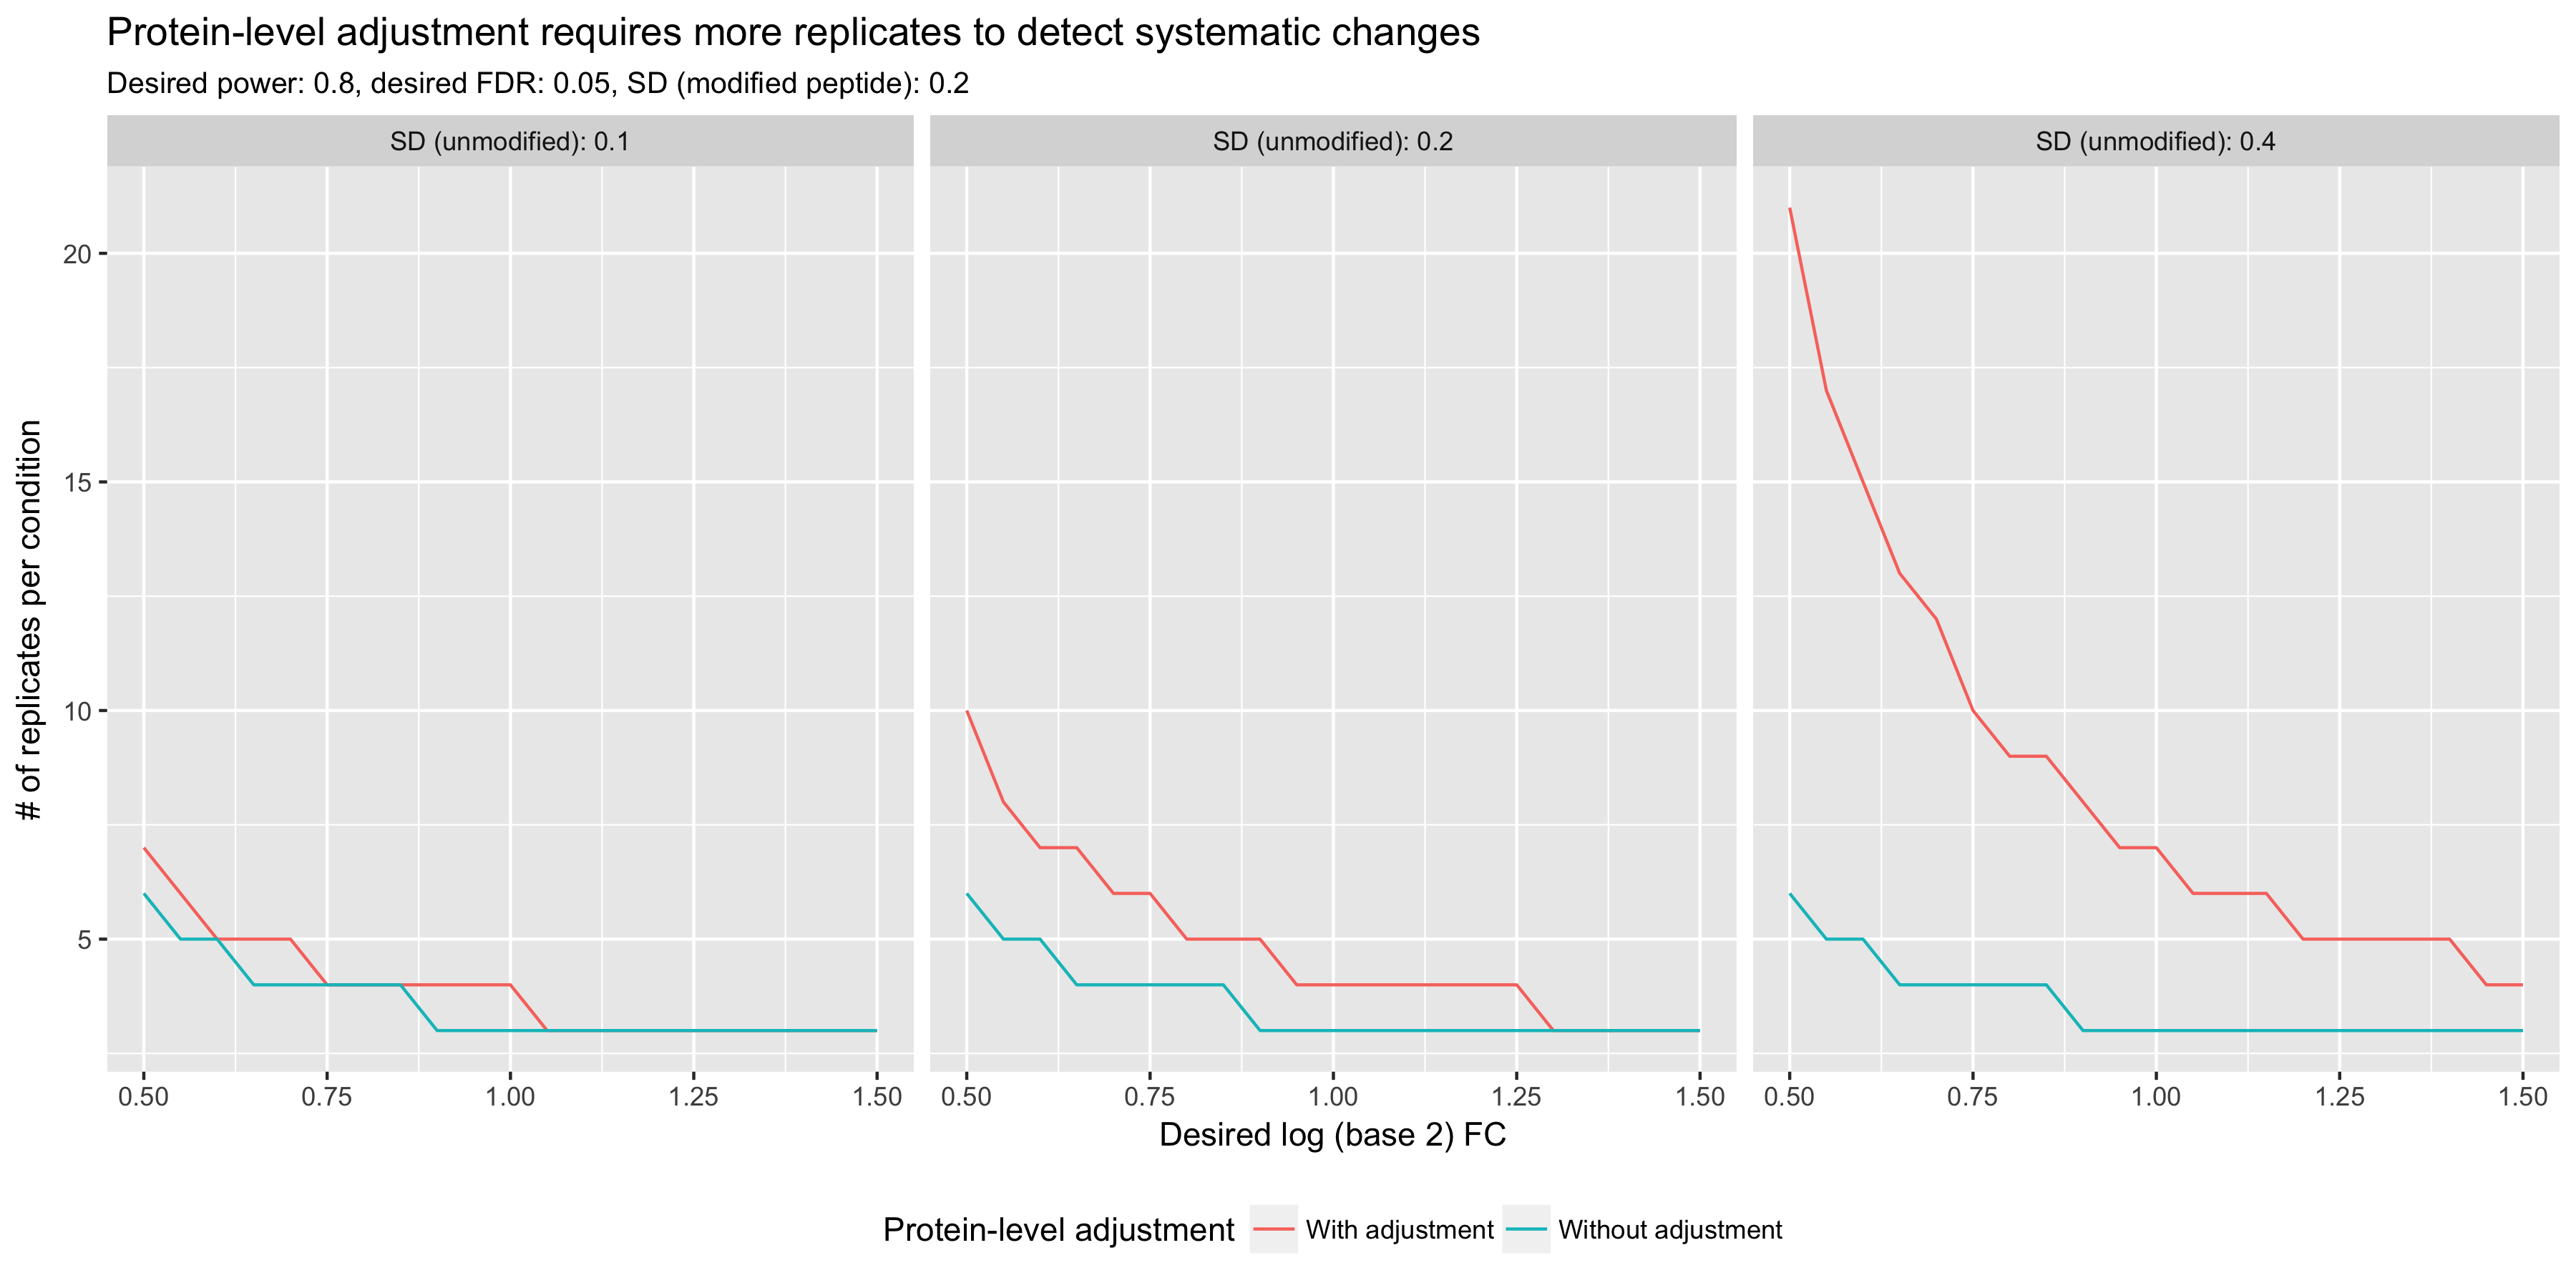
\includegraphics[width=\textwidth]{sim/size_prot}
%\caption{Protein-level adjustment relies on the inference of protein abundance, %which introduces additional uncertainty in the estimate of PTM difference. %Therefore, the required sample size to detect a systematic change is higher than as %expected for standard differential analysis without adjustment. The discrepancy can %be profound if the uncertainty associated with the protein abundance estimate is %greater than that of PTM abundance estimate. Sample size calculation without %accounting for the uncertainty would lead to under-powered studies. %\label{fig:size_prot}}
%\end{figure}

%\begin{figure}[h!]
%\centering
%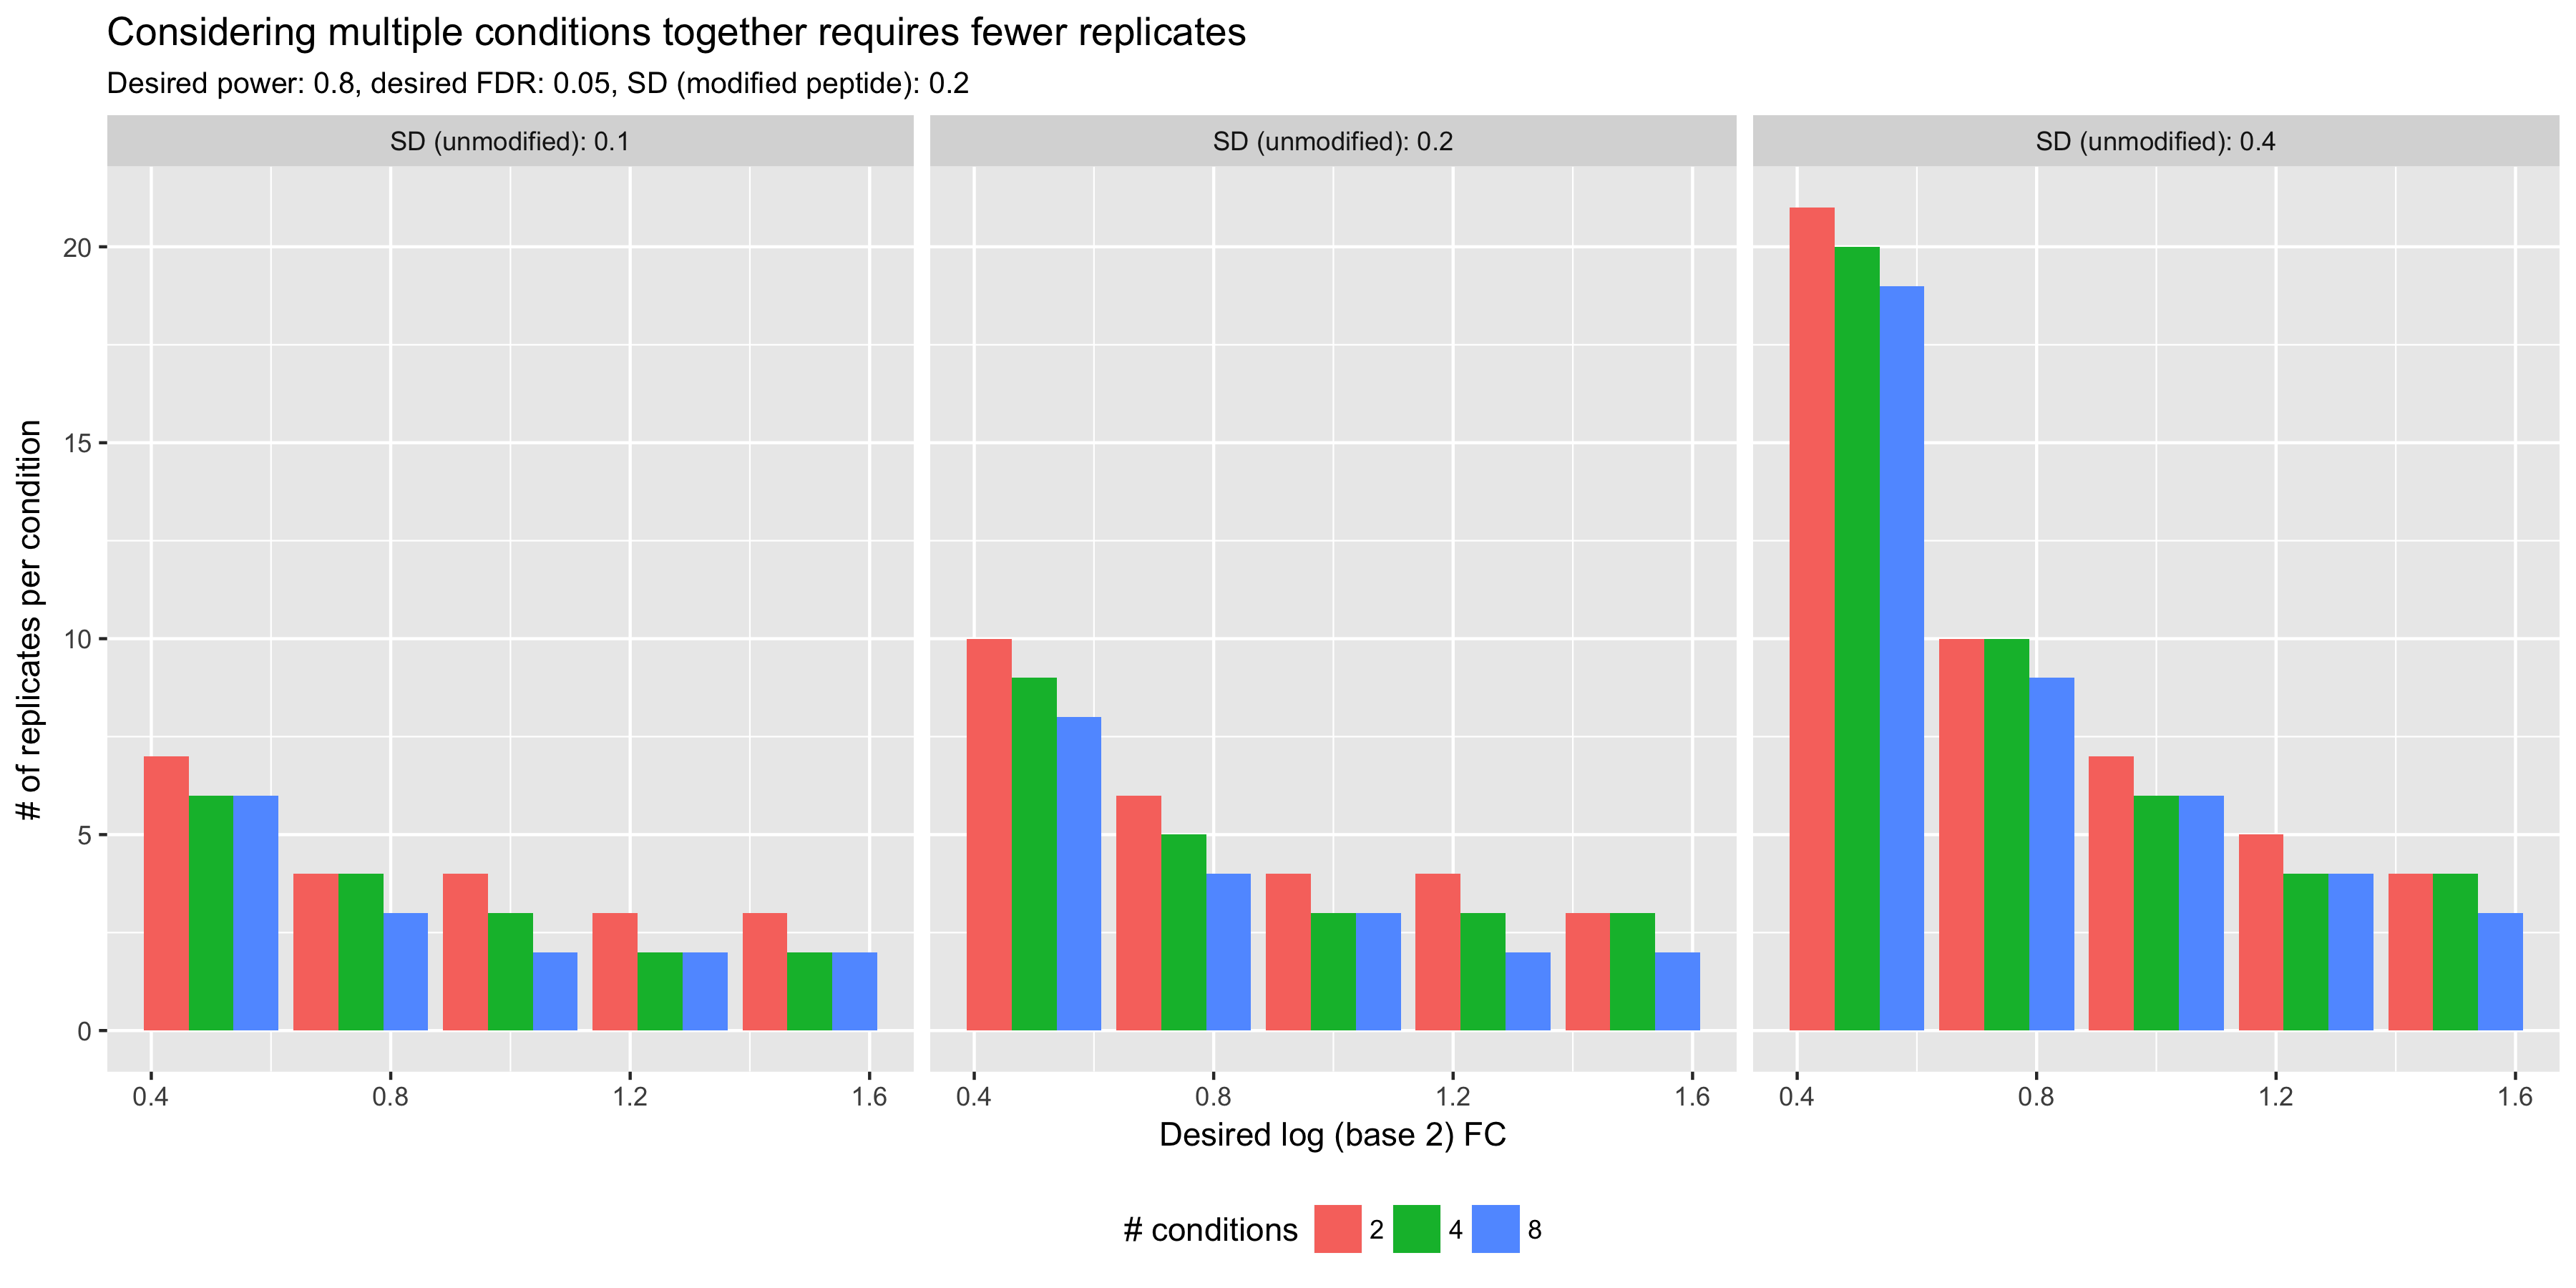
\includegraphics[width=\textwidth]{sim/size_grp}
%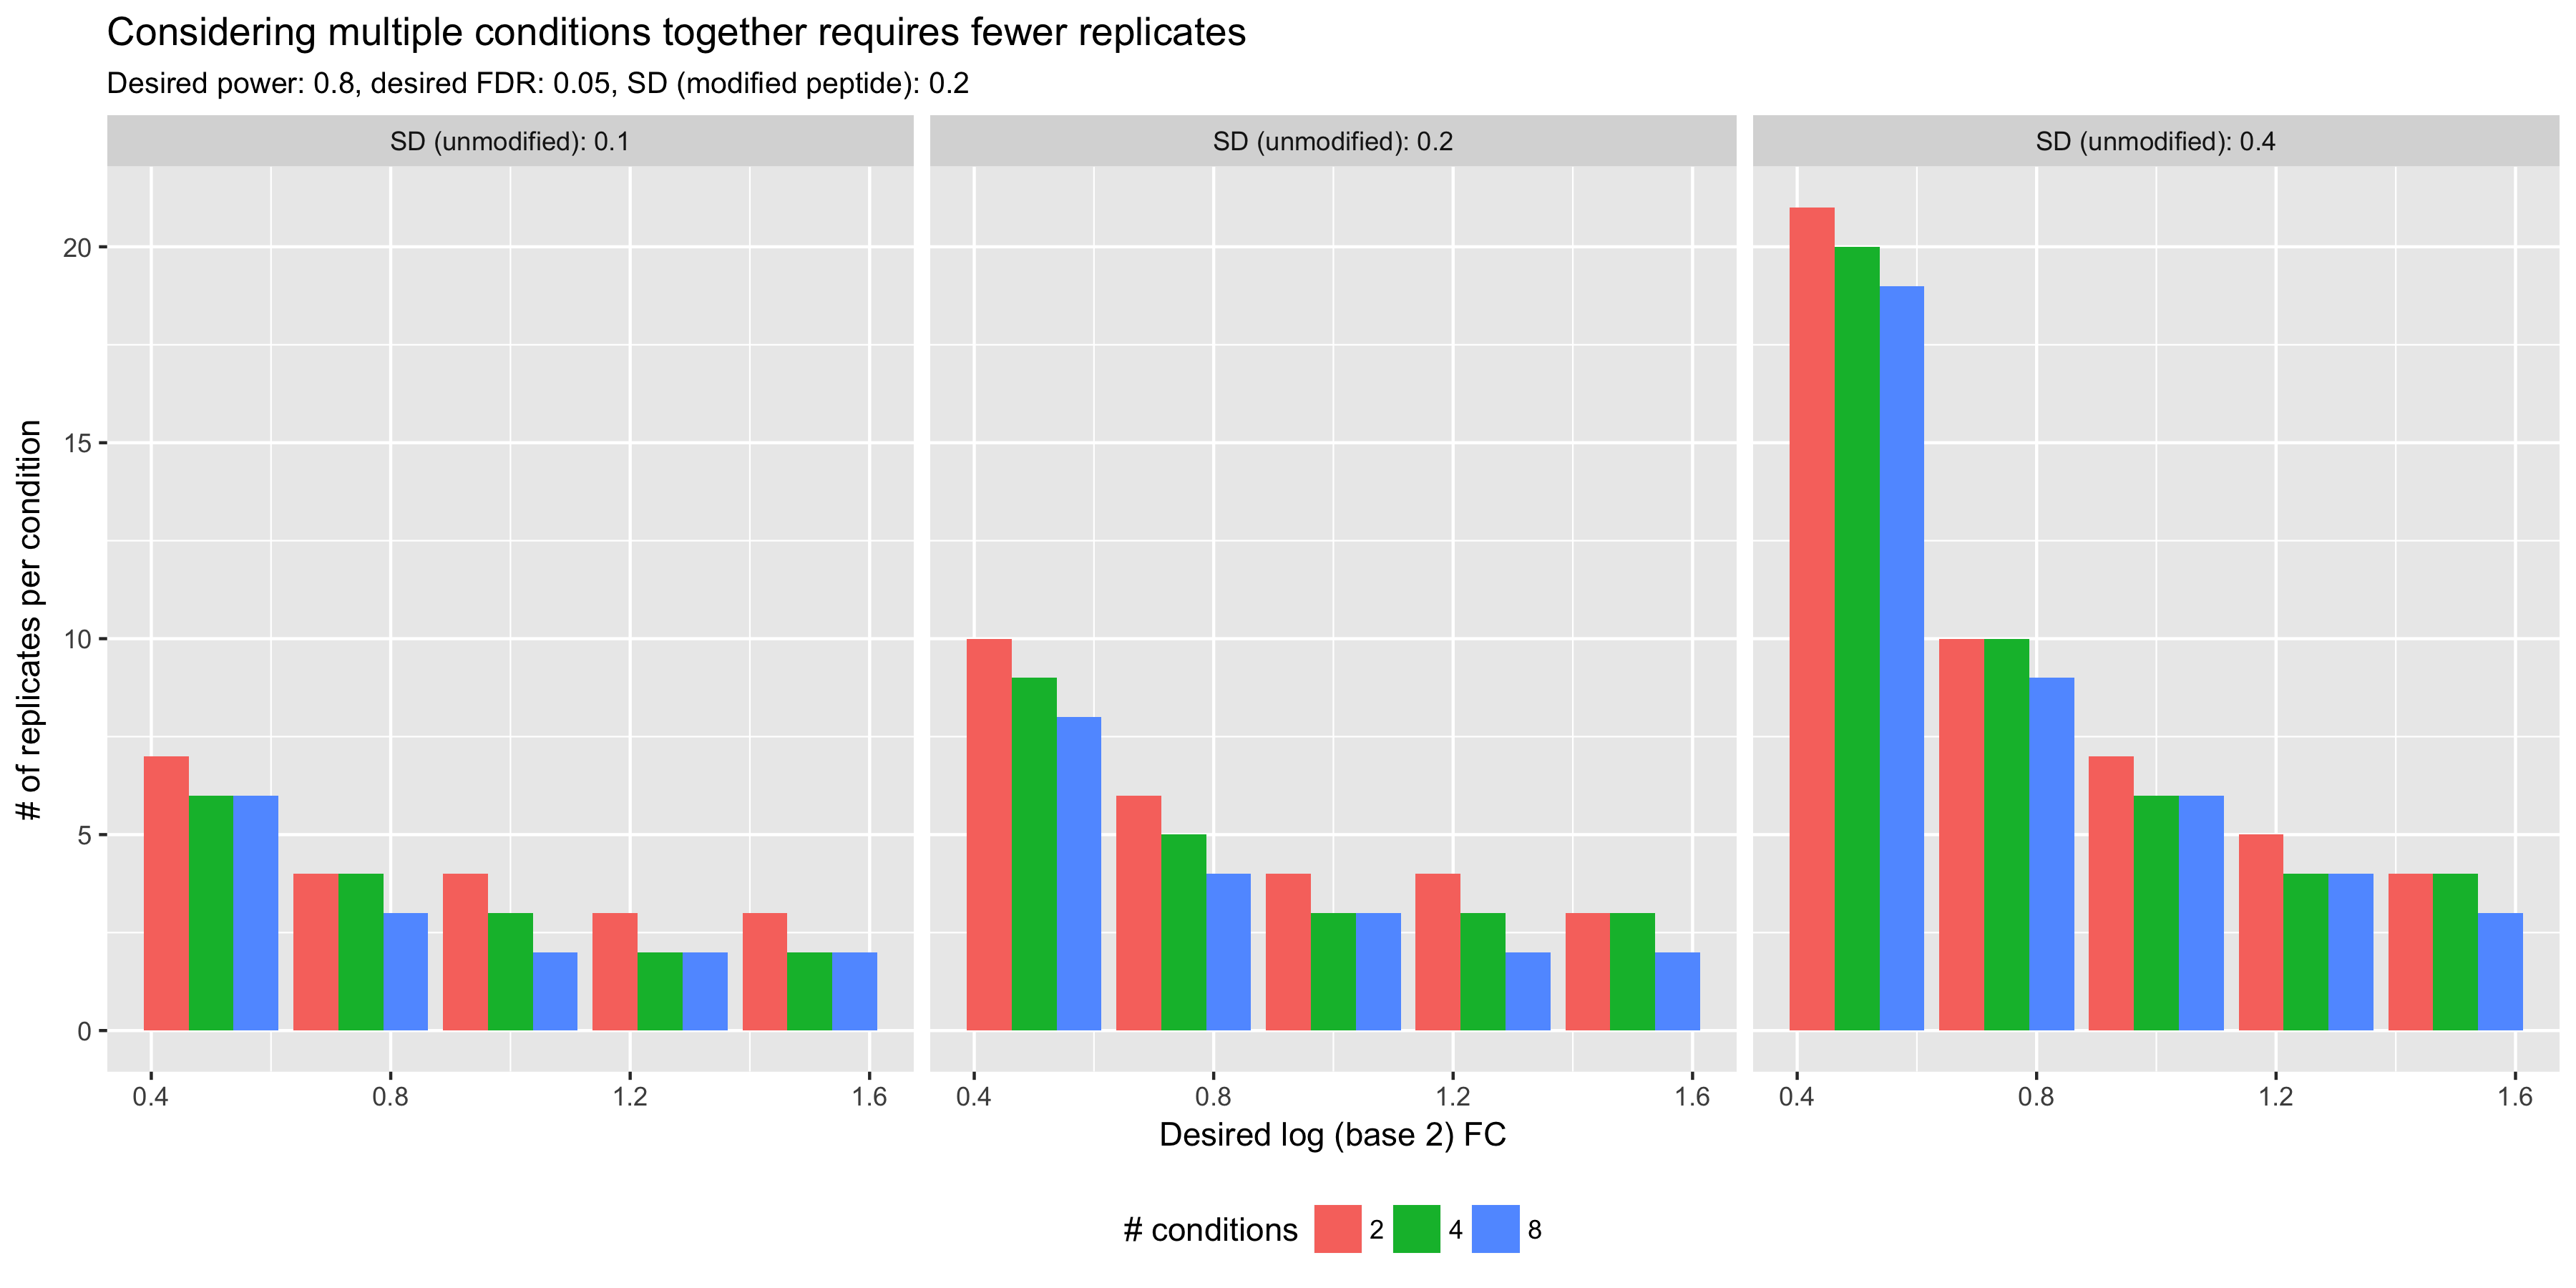
\includegraphics[width=.725\textwidth]{sim/size_grp}
%\caption{In complex designs, simultaneously analyzing all the conditions% effectively increases the degrees of freedom and requires fewer replicates. %\label{fig:size_grp}}
%\end{figure}

%\begin{figure}[h!]
%\centering
%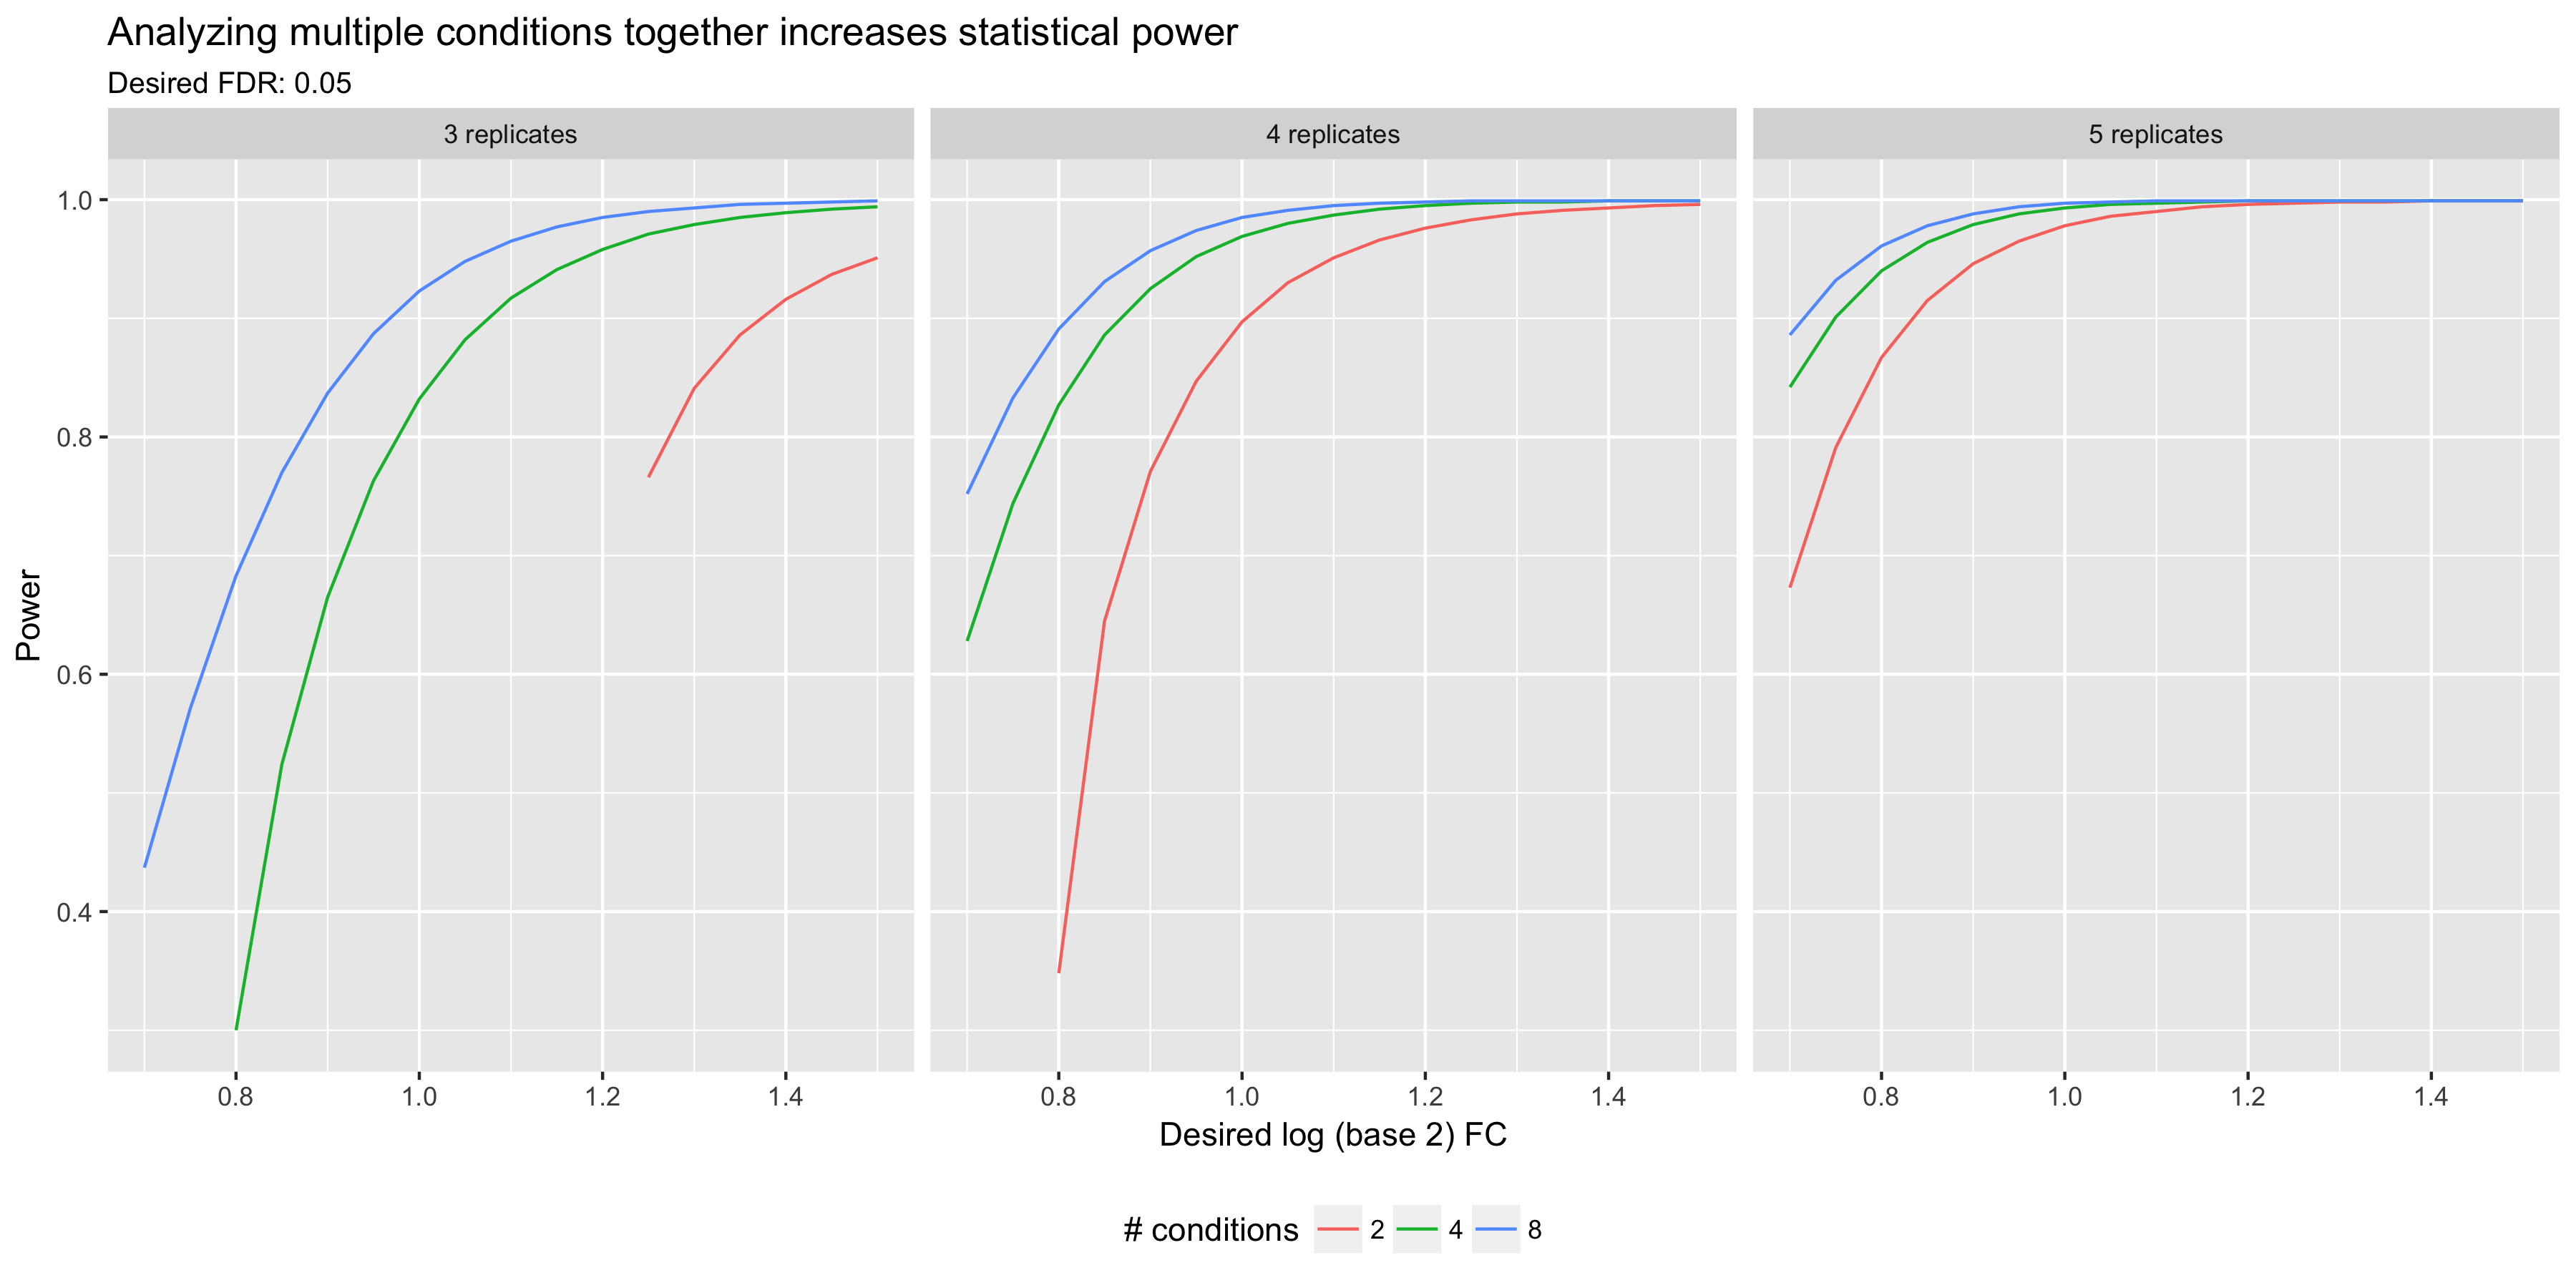
\includegraphics[width=\textwidth]{sim/pwr_grp}
%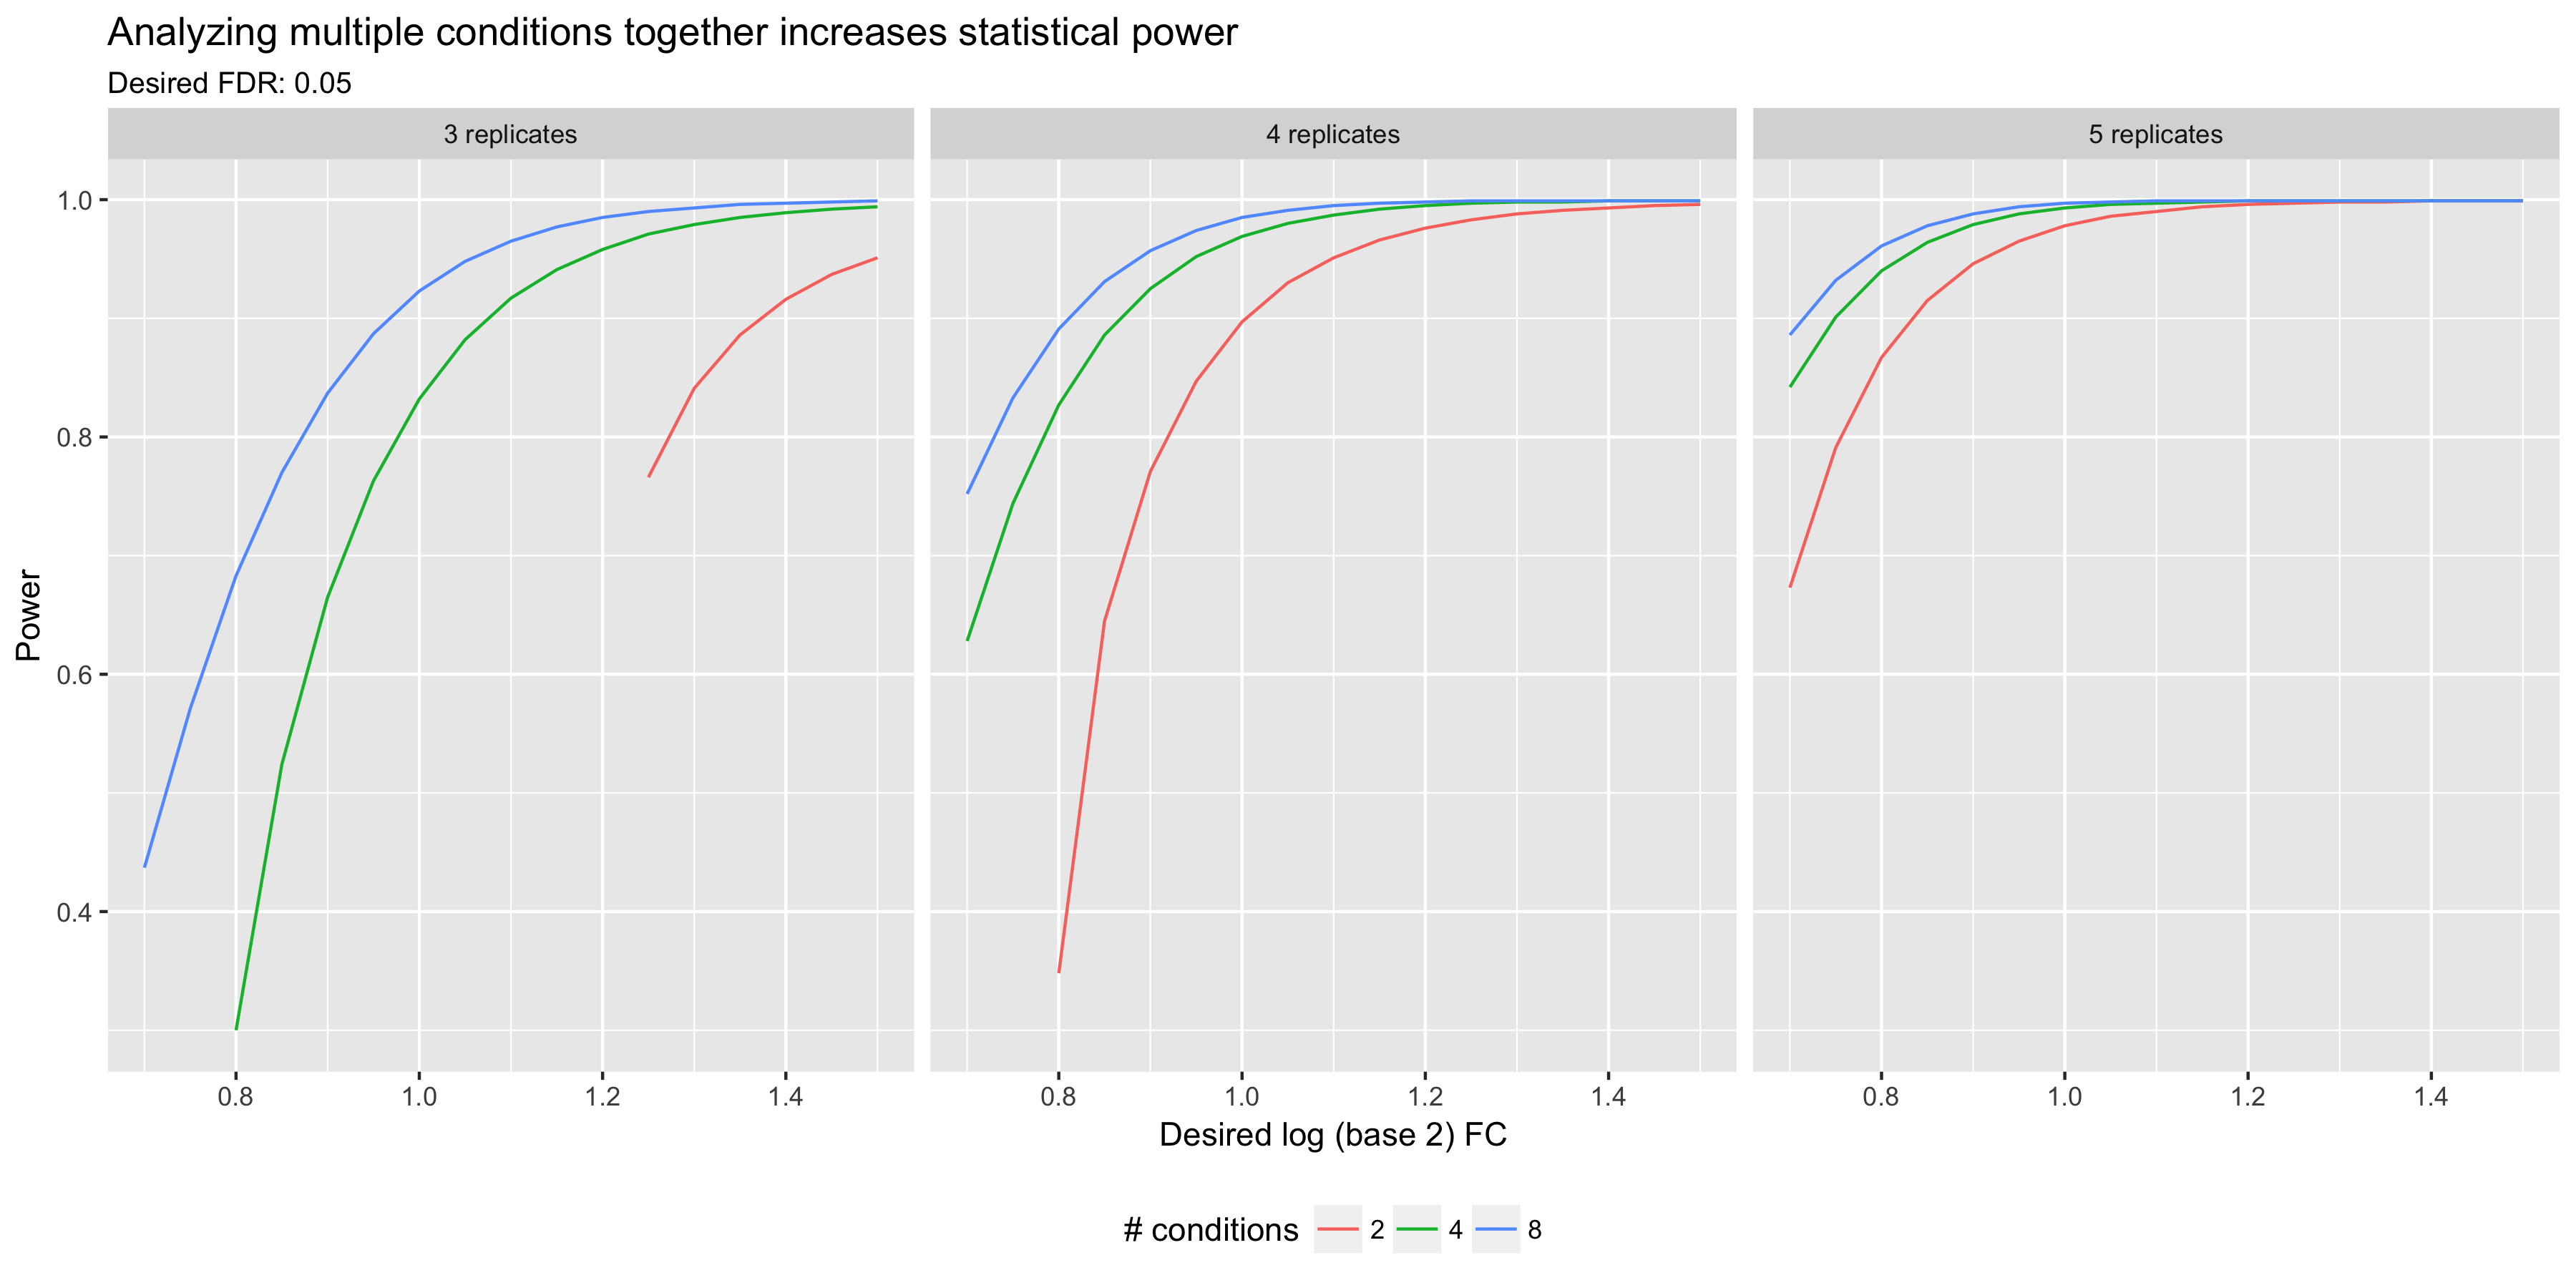
\includegraphics[width=.725\textwidth]{sim/pwr_grp}
%\caption{Statistical power can be improved by increasing the sample size and %analyzing multiple conditions together. \label{fig:pwr_grp}}
%\end{figure}



%%%%%%%%%%%%%%%%%%%%%%%%%%%%%%%%%%%%%%%%%%%%%%%%%%%%%%%%%%%%%%%%
%\clearpage

%\printbibliography 

\end{document} 

